\documentclass[letterpaper,12pt]{article}
%% Language and font encodings
\usepackage[english]{babel}
\usepackage[utf8x]{inputenc}
\usepackage[T1]{fontenc}
\usepackage{titlesec}
\setcounter{secnumdepth}{4}
\usepackage{alphalph}

\titlespacing\section{0pt}{8pt plus 0pt minus 0pt}{2pt plus 0pt minus 0pt}
\titlespacing\subsection{0pt}{8pt plus 0pt minus 0pt}{2pt plus 0pt minus 0pt}
\titlespacing\subsubsection{0pt}{8pt plus 0pt minus 0pt}{2pt plus 0pt minus 0pt}

%% Sets page size and margins
\usepackage[letterpaper,top=1in,bottom=1in,left=1in,right=1in,marginparwidth=0in]{geometry}
\usepackage{soul} % for underlining text

% set font
% see https://www.sharelatex.com/learn/Font_typefaces (halfway down) for options
% put the package name (2nd column at website) in line 14 and put the fontcode (3rd column at website) in {} on line 29 in \fontfamily
\usepackage{times}

%% Useful packages
\usepackage{amsmath}
\usepackage{graphicx}
\usepackage[colorinlistoftodos]{todonotes}
\usepackage[colorlinks=true, allcolors=blue]{hyperref}
%\usepackage[colorlinks=true, allcolors=black]{hyperref}

\usepackage{multirow} % for tables
\usepackage{xcolor,colortbl} % for tables
\usepackage{enumitem} % for lists
\usepackage{natbib} % allows for alias in citations, i.e., inputing a different name to show up in the document if the full name is super long and runs off the page.
\usepackage{libertine} % for getting ug/m3 
\usepackage{float}

\newcommand*{\brokenurl}[2]{\href{#1#2}{\texttt{#1}}\par\nopagebreak\href{#1#2}{\texttt{#2}}}
\newcommand*{\brokenurlwithoutpar}[2]{\href{#1#2}{\texttt{#1}}\\*\href{#1#2}{\texttt{#2}}}

\begin{document}
\fontfamily{ptm}\selectfont
\urlstyle{same}
\urlstyle{rm}

\tableofcontents

\pagebreak

%
\section{Report PM2.5 part e Data Version: Include All Monitors} 
 

\begin{figure} 
\centering  
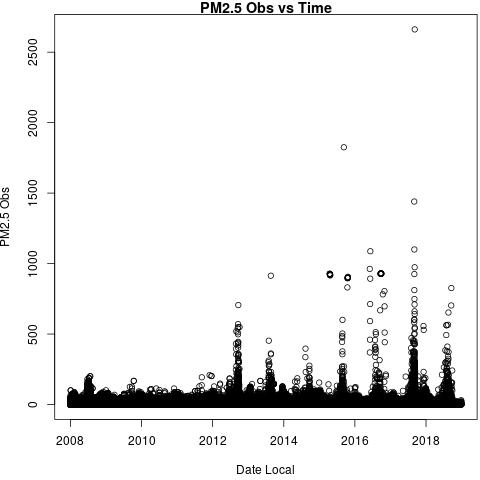
\includegraphics[width=0.77\textwidth]{Code_Outputs/Report_PM25_Step4_part_e_de_duplicated_aves_ML_input_PM25_ObsvDate_Local.jpg} 
\caption{\label{fig:Report_PM25_Step4_part_e_de_duplicated_aves_ML_inputPM25_ObsvDate_Local}vs Time} 
\end{figure} 
 

\begin{figure} 
\centering  
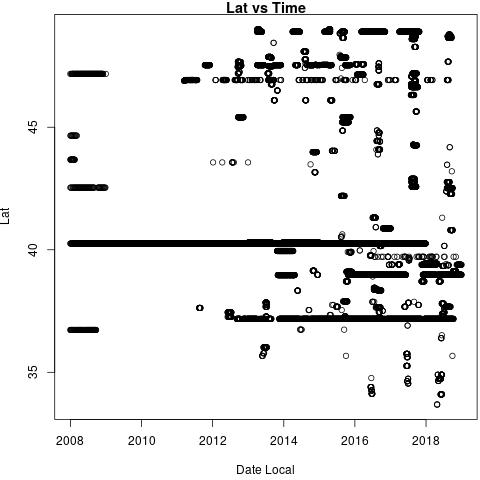
\includegraphics[width=0.77\textwidth]{Code_Outputs/Report_PM25_Step4_part_e_de_duplicated_aves_ML_input_LatvDate_Local.jpg} 
\caption{\label{fig:Report_PM25_Step4_part_e_de_duplicated_aves_ML_inputLatvDate_Local}vs Time} 
\end{figure} 
 

\begin{figure} 
\centering  
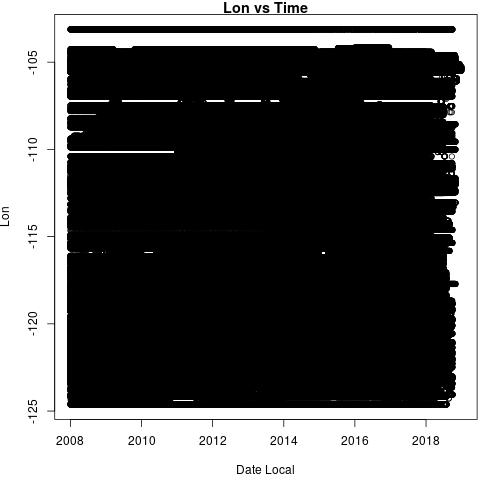
\includegraphics[width=0.77\textwidth]{Code_Outputs/Report_PM25_Step4_part_e_de_duplicated_aves_ML_input_LonvDate_Local.jpg} 
\caption{\label{fig:Report_PM25_Step4_part_e_de_duplicated_aves_ML_inputLonvDate_Local}vs Time} 
\end{figure} 
 

\begin{figure} 
\centering  
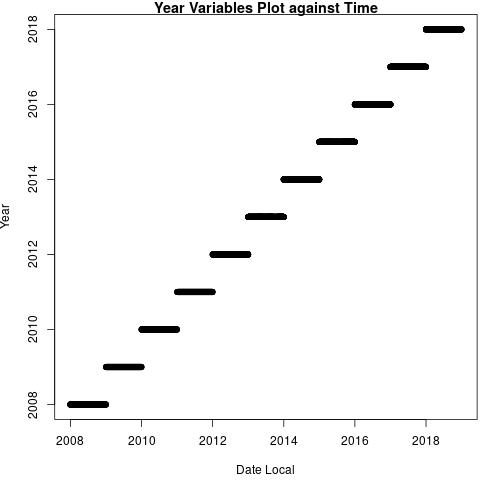
\includegraphics[width=0.77\textwidth]{Code_Outputs/Report_PM25_Step4_part_e_de_duplicated_aves_ML_input_YearvDate_Local.jpg} 
\caption{\label{fig:Report_PM25_Step4_part_e_de_duplicated_aves_ML_inputYearvDate_Local}vs Time} 
\end{figure} 
 

\begin{figure} 
\centering  
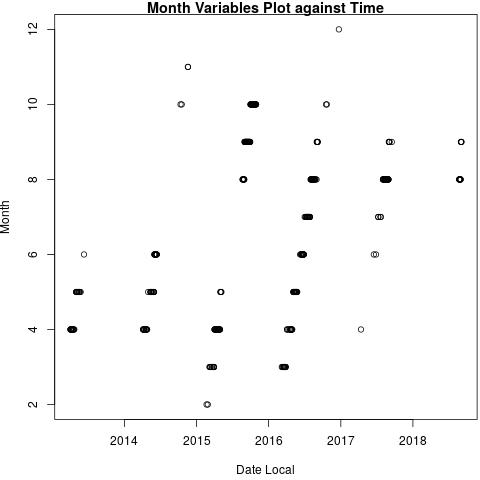
\includegraphics[width=0.77\textwidth]{Code_Outputs/Report_PM25_Step4_part_e_de_duplicated_aves_ML_input_MonthvDate_Local.jpg} 
\caption{\label{fig:Report_PM25_Step4_part_e_de_duplicated_aves_ML_inputMonthvDate_Local}vs Time} 
\end{figure} 
 

\begin{figure} 
\centering  
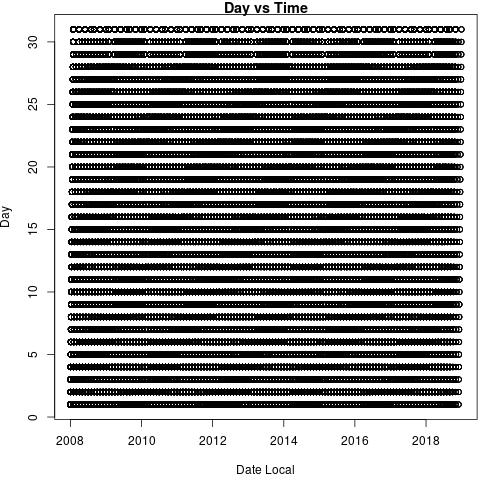
\includegraphics[width=0.77\textwidth]{Code_Outputs/Report_PM25_Step4_part_e_de_duplicated_aves_ML_input_DayvDate_Local.jpg} 
\caption{\label{fig:Report_PM25_Step4_part_e_de_duplicated_aves_ML_inputDayvDate_Local}vs Time} 
\end{figure} 
 

\begin{figure} 
\centering  
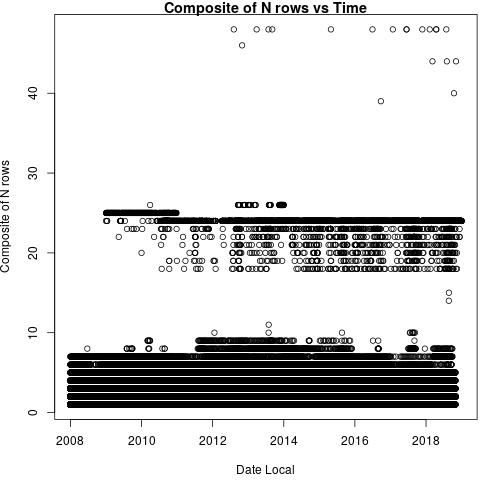
\includegraphics[width=0.77\textwidth]{Code_Outputs/Report_PM25_Step4_part_e_de_duplicated_aves_ML_input_Composite_of_N_rowsvDate_Local.jpg} 
\caption{\label{fig:Report_PM25_Step4_part_e_de_duplicated_aves_ML_inputComposite_of_N_rowsvDate_Local}vs Time} 
\end{figure} 
 

\begin{figure} 
\centering  
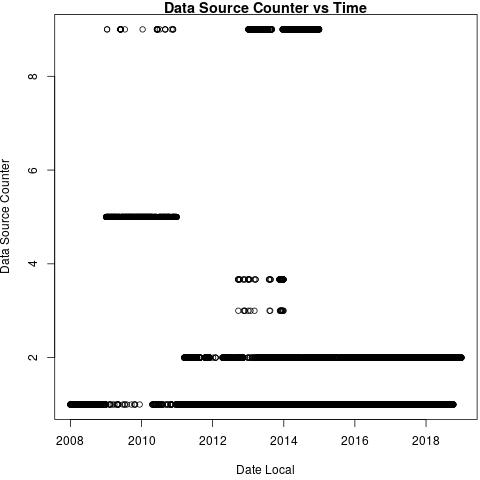
\includegraphics[width=0.77\textwidth]{Code_Outputs/Report_PM25_Step4_part_e_de_duplicated_aves_ML_input_Data_Source_CountervDate_Local.jpg} 
\caption{\label{fig:Report_PM25_Step4_part_e_de_duplicated_aves_ML_inputData_Source_CountervDate_Local}vs Time} 
\end{figure} 
 

\begin{figure} 
\centering  
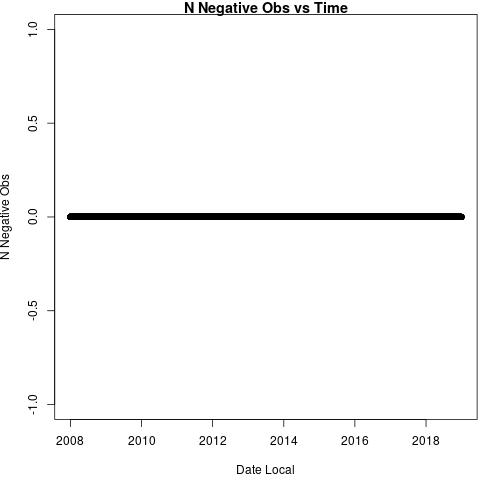
\includegraphics[width=0.77\textwidth]{Code_Outputs/Report_PM25_Step4_part_e_de_duplicated_aves_ML_input_N_Negative_ObsvDate_Local.jpg} 
\caption{\label{fig:Report_PM25_Step4_part_e_de_duplicated_aves_ML_inputN_Negative_ObsvDate_Local}vs Time} 
\end{figure} 
 

\clearpage 

\begin{figure} 
\centering  
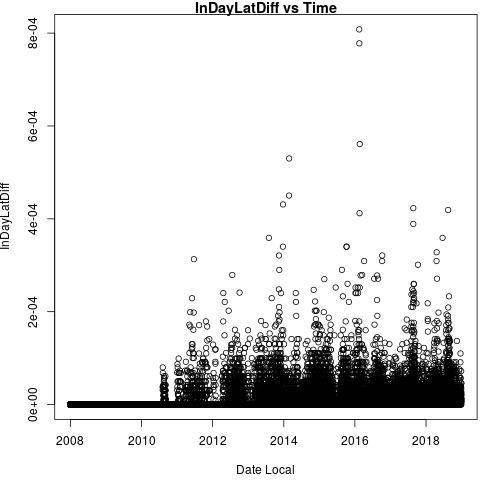
\includegraphics[width=0.77\textwidth]{Code_Outputs/Report_PM25_Step4_part_e_de_duplicated_aves_ML_input_InDayLatDiffvDate_Local.jpg} 
\caption{\label{fig:Report_PM25_Step4_part_e_de_duplicated_aves_ML_inputInDayLatDiffvDate_Local}vs Time} 
\end{figure} 
 

\begin{figure} 
\centering  
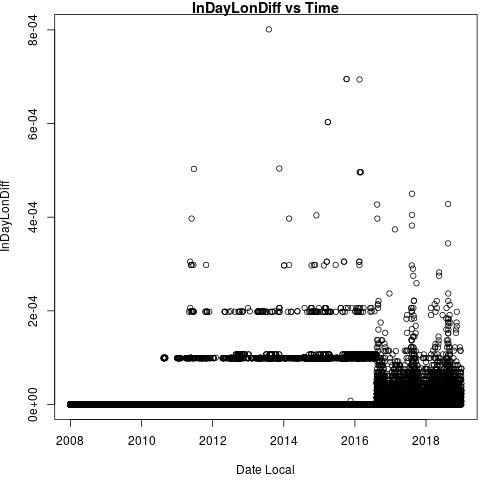
\includegraphics[width=0.77\textwidth]{Code_Outputs/Report_PM25_Step4_part_e_de_duplicated_aves_ML_input_InDayLonDiffvDate_Local.jpg} 
\caption{\label{fig:Report_PM25_Step4_part_e_de_duplicated_aves_ML_inputInDayLonDiffvDate_Local}vs Time} 
\end{figure} 
 

\subsection{All PM2.5 Monitor Locations Images} 
 

\begin{figure} 
\centering  
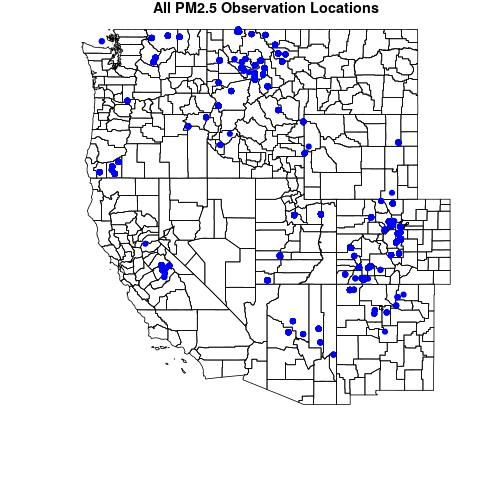
\includegraphics[width=0.77\textwidth]{Code_Outputs/Report_PM25_Step4_part_e_de_duplicated_aves_ML_input_PlotLoc0.jpg} 
\caption{\label{fig:Report_PM25_Step4_part_e_de_duplicated_aves_ML_inputPlotLoc0}All PM2.5 Observation Locations} 
\end{figure} 
 

\begin{figure} 
\centering  
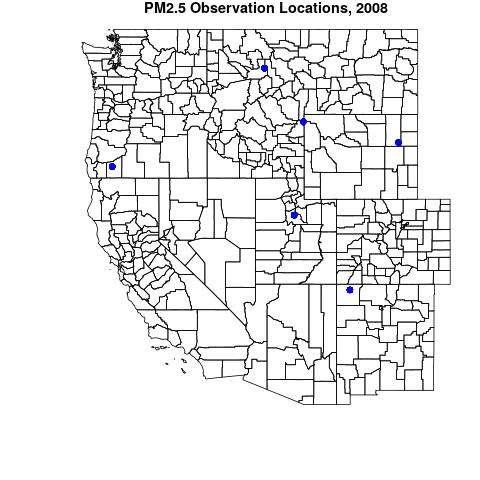
\includegraphics[width=0.77\textwidth]{Code_Outputs/Report_PM25_Step4_part_e_de_duplicated_aves_ML_input_PlotLoc2008.jpg} 
\caption{\label{fig:Report_PM25_Step4_part_e_de_duplicated_aves_ML_inputPlotLoc2008}PM2.5 Observation Locations, 2008} 
\end{figure} 
 

\begin{figure} 
\centering  
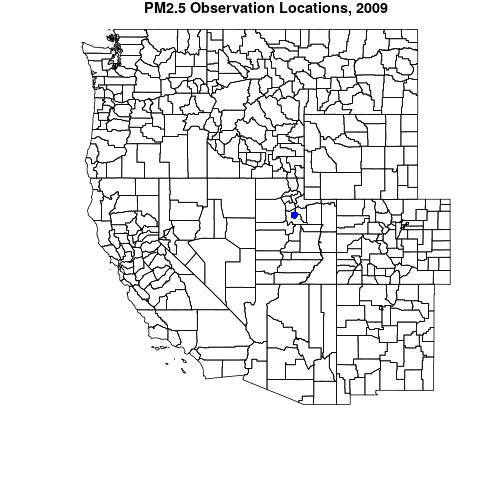
\includegraphics[width=0.77\textwidth]{Code_Outputs/Report_PM25_Step4_part_e_de_duplicated_aves_ML_input_PlotLoc2009.jpg} 
\caption{\label{fig:Report_PM25_Step4_part_e_de_duplicated_aves_ML_inputPlotLoc2009}PM2.5 Observation Locations, 2009} 
\end{figure} 
 

\begin{figure} 
\centering  
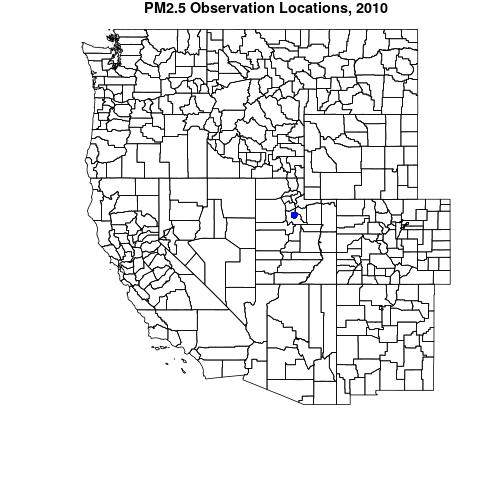
\includegraphics[width=0.77\textwidth]{Code_Outputs/Report_PM25_Step4_part_e_de_duplicated_aves_ML_input_PlotLoc2010.jpg} 
\caption{\label{fig:Report_PM25_Step4_part_e_de_duplicated_aves_ML_inputPlotLoc2010}PM2.5 Observation Locations, 2010} 
\end{figure} 
 

\begin{figure} 
\centering  
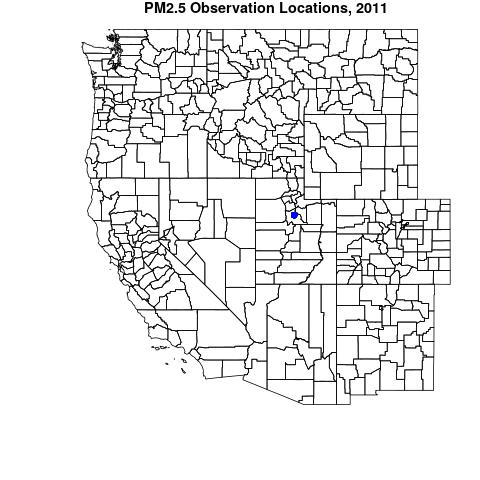
\includegraphics[width=0.77\textwidth]{Code_Outputs/Report_PM25_Step4_part_e_de_duplicated_aves_ML_input_PlotLoc2011.jpg} 
\caption{\label{fig:Report_PM25_Step4_part_e_de_duplicated_aves_ML_inputPlotLoc2011}PM2.5 Observation Locations, 2011} 
\end{figure} 
 

\begin{figure} 
\centering  
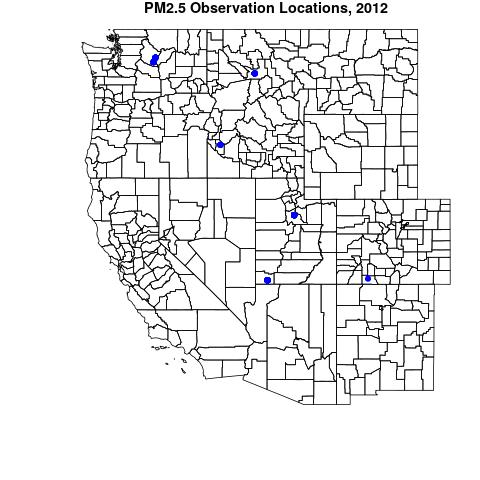
\includegraphics[width=0.77\textwidth]{Code_Outputs/Report_PM25_Step4_part_e_de_duplicated_aves_ML_input_PlotLoc2012.jpg} 
\caption{\label{fig:Report_PM25_Step4_part_e_de_duplicated_aves_ML_inputPlotLoc2012}PM2.5 Observation Locations, 2012} 
\end{figure} 
 

\begin{figure} 
\centering  
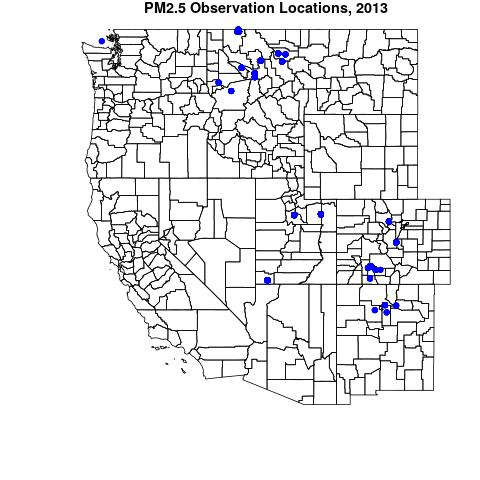
\includegraphics[width=0.77\textwidth]{Code_Outputs/Report_PM25_Step4_part_e_de_duplicated_aves_ML_input_PlotLoc2013.jpg} 
\caption{\label{fig:Report_PM25_Step4_part_e_de_duplicated_aves_ML_inputPlotLoc2013}PM2.5 Observation Locations, 2013} 
\end{figure} 
 

\begin{figure} 
\centering  
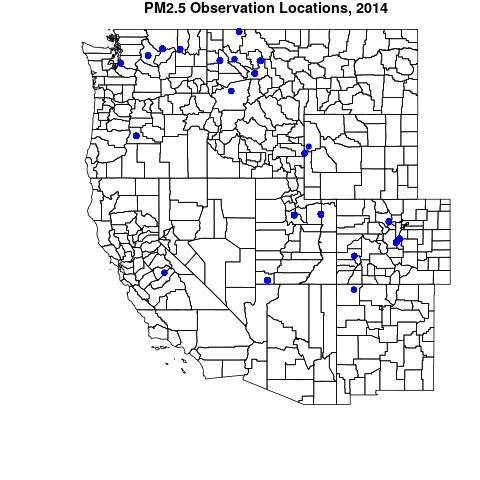
\includegraphics[width=0.77\textwidth]{Code_Outputs/Report_PM25_Step4_part_e_de_duplicated_aves_ML_input_PlotLoc2014.jpg} 
\caption{\label{fig:Report_PM25_Step4_part_e_de_duplicated_aves_ML_inputPlotLoc2014}PM2.5 Observation Locations, 2014} 
\end{figure} 
 

\begin{figure} 
\centering  
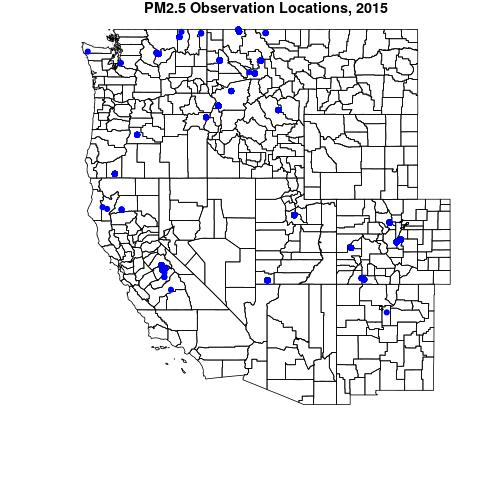
\includegraphics[width=0.77\textwidth]{Code_Outputs/Report_PM25_Step4_part_e_de_duplicated_aves_ML_input_PlotLoc2015.jpg} 
\caption{\label{fig:Report_PM25_Step4_part_e_de_duplicated_aves_ML_inputPlotLoc2015}PM2.5 Observation Locations, 2015} 
\end{figure} 
 

\begin{figure} 
\centering  
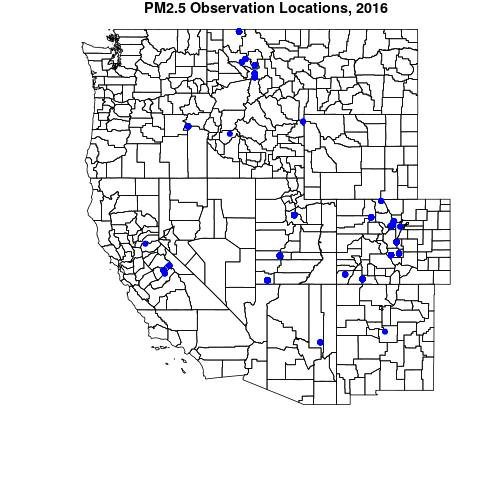
\includegraphics[width=0.77\textwidth]{Code_Outputs/Report_PM25_Step4_part_e_de_duplicated_aves_ML_input_PlotLoc2016.jpg} 
\caption{\label{fig:Report_PM25_Step4_part_e_de_duplicated_aves_ML_inputPlotLoc2016}PM2.5 Observation Locations, 2016} 
\end{figure} 
 

\begin{figure} 
\centering  
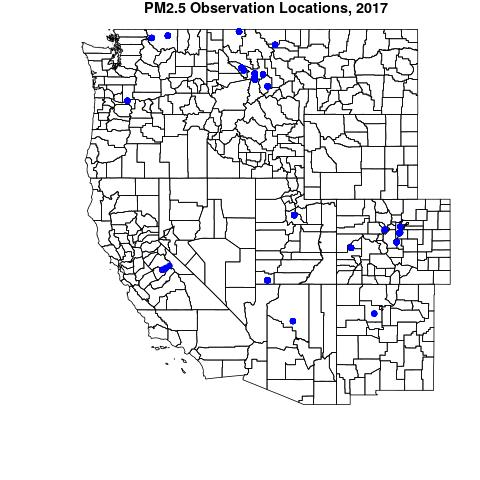
\includegraphics[width=0.77\textwidth]{Code_Outputs/Report_PM25_Step4_part_e_de_duplicated_aves_ML_input_PlotLoc2017.jpg} 
\caption{\label{fig:Report_PM25_Step4_part_e_de_duplicated_aves_ML_inputPlotLoc2017}PM2.5 Observation Locations, 2017} 
\end{figure} 
 

\begin{figure} 
\centering  
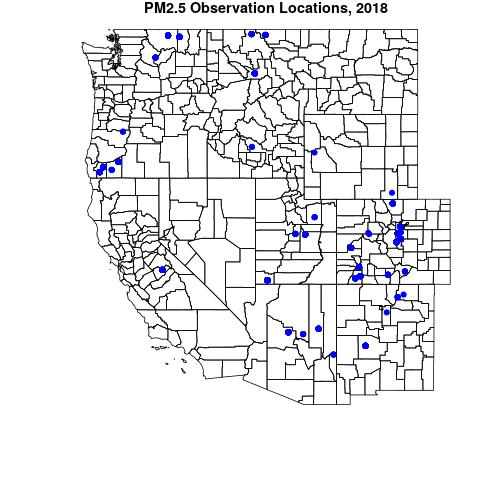
\includegraphics[width=0.77\textwidth]{Code_Outputs/Report_PM25_Step4_part_e_de_duplicated_aves_ML_input_PlotLoc2018.jpg} 
\caption{\label{fig:Report_PM25_Step4_part_e_de_duplicated_aves_ML_inputPlotLoc2018}PM2.5 Observation Locations, 2018} 
\end{figure} 
 
 % UNCOMMENT?

% Time series for each predictor variable

\subsection{ML Inputs Time Series Images} 
 

\begin{figure} 
\centering  
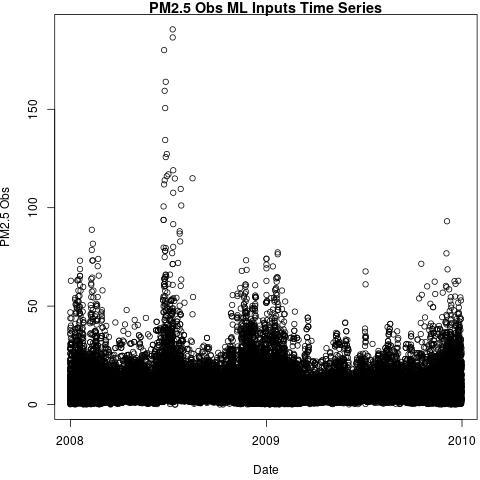
\includegraphics[width=0.77\textwidth]{Code_Outputs/Report_ML_input_PM25_Step4_part_e_de_duplicated_aves_PM25_ObsvDate.jpg} 
\caption{\label{fig:Report_ML_input_PM25_Step4_part_e_de_duplicated_avesPM25_ObsvDate}ML Inputs Time Series} 
\end{figure} 
 

\begin{figure} 
\centering  
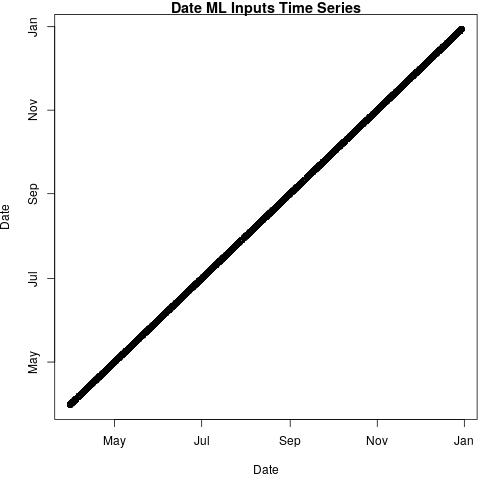
\includegraphics[width=0.77\textwidth]{Code_Outputs/Report_ML_input_PM25_Step4_part_e_de_duplicated_aves_DatevDate.jpg} 
\caption{\label{fig:Report_ML_input_PM25_Step4_part_e_de_duplicated_avesDatevDate}ML Inputs Time Series} 
\end{figure} 
 

\begin{figure} 
\centering  
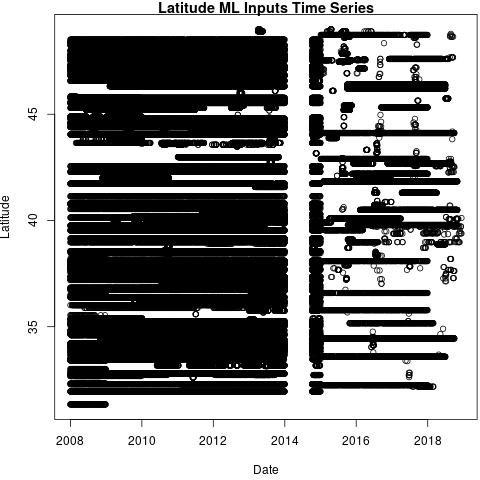
\includegraphics[width=0.77\textwidth]{Code_Outputs/Report_ML_input_PM25_Step4_part_e_de_duplicated_aves_LatitudevDate.jpg} 
\caption{\label{fig:Report_ML_input_PM25_Step4_part_e_de_duplicated_avesLatitudevDate}ML Inputs Time Series} 
\end{figure} 
 

\begin{figure} 
\centering  
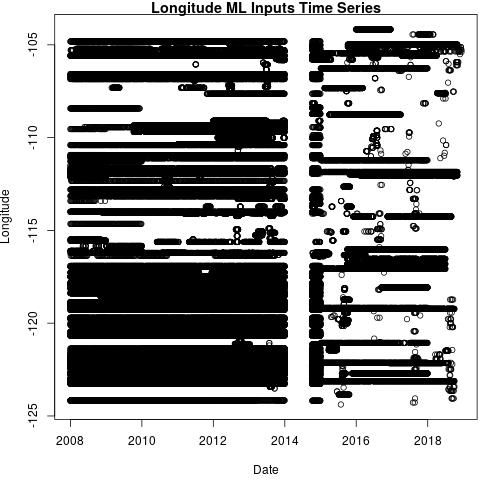
\includegraphics[width=0.77\textwidth]{Code_Outputs/Report_ML_input_PM25_Step4_part_e_de_duplicated_aves_LongitudevDate.jpg} 
\caption{\label{fig:Report_ML_input_PM25_Step4_part_e_de_duplicated_avesLongitudevDate}ML Inputs Time Series} 
\end{figure} 
 

\begin{figure} 
\centering  
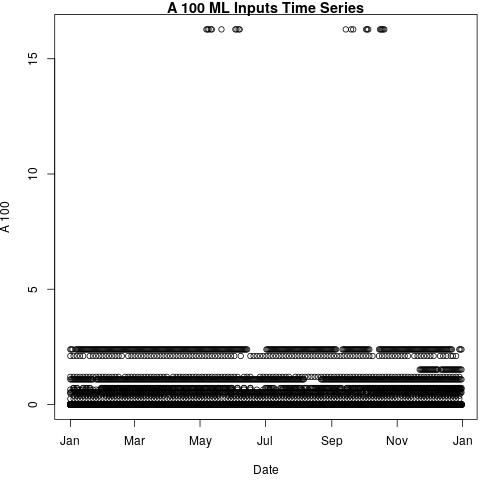
\includegraphics[width=0.77\textwidth]{Code_Outputs/Report_ML_input_PM25_Step4_part_e_de_duplicated_aves_A_100vDate.jpg} 
\caption{\label{fig:Report_ML_input_PM25_Step4_part_e_de_duplicated_avesA_100vDate}ML Inputs Time Series} 
\end{figure} 
 

\begin{figure} 
\centering  
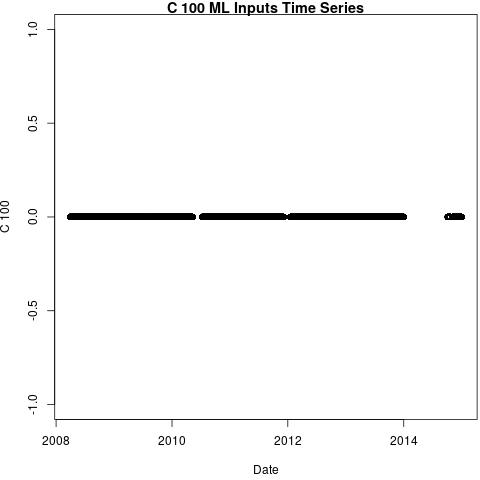
\includegraphics[width=0.77\textwidth]{Code_Outputs/Report_ML_input_PM25_Step4_part_e_de_duplicated_aves_C_100vDate.jpg} 
\caption{\label{fig:Report_ML_input_PM25_Step4_part_e_de_duplicated_avesC_100vDate}ML Inputs Time Series} 
\end{figure} 
 

\begin{figure} 
\centering  
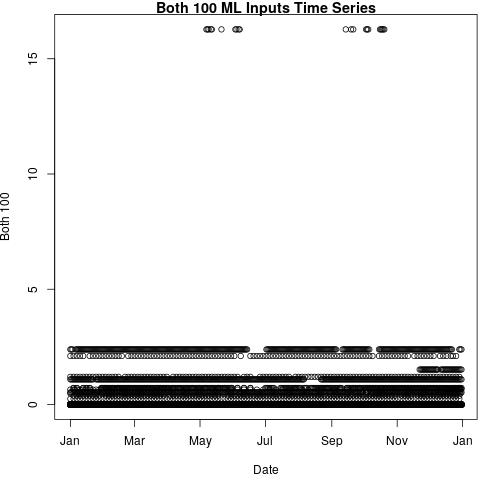
\includegraphics[width=0.77\textwidth]{Code_Outputs/Report_ML_input_PM25_Step4_part_e_de_duplicated_aves_Both_100vDate.jpg} 
\caption{\label{fig:Report_ML_input_PM25_Step4_part_e_de_duplicated_avesBoth_100vDate}ML Inputs Time Series} 
\end{figure} 
 

\begin{figure} 
\centering  
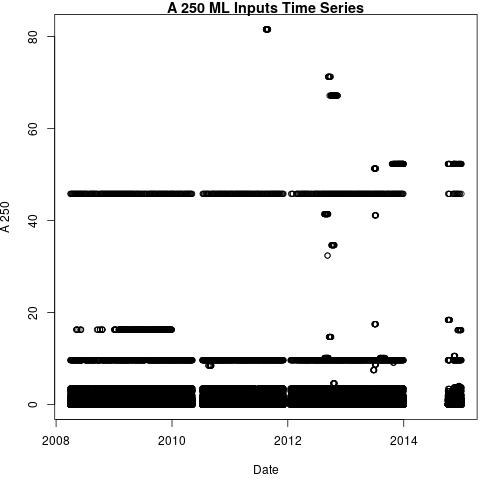
\includegraphics[width=0.77\textwidth]{Code_Outputs/Report_ML_input_PM25_Step4_part_e_de_duplicated_aves_A_250vDate.jpg} 
\caption{\label{fig:Report_ML_input_PM25_Step4_part_e_de_duplicated_avesA_250vDate}ML Inputs Time Series} 
\end{figure} 
 

\begin{figure} 
\centering  
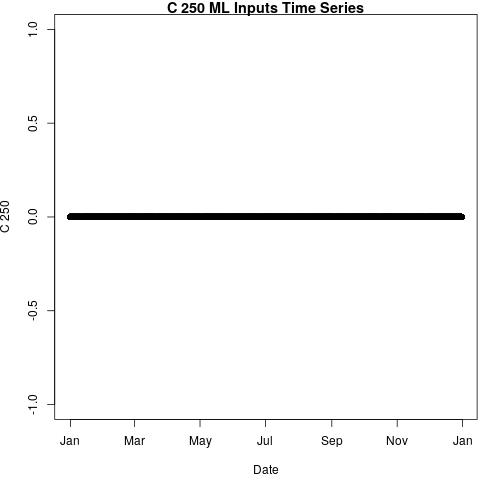
\includegraphics[width=0.77\textwidth]{Code_Outputs/Report_ML_input_PM25_Step4_part_e_de_duplicated_aves_C_250vDate.jpg} 
\caption{\label{fig:Report_ML_input_PM25_Step4_part_e_de_duplicated_avesC_250vDate}ML Inputs Time Series} 
\end{figure} 
 

\clearpage 

\begin{figure} 
\centering  
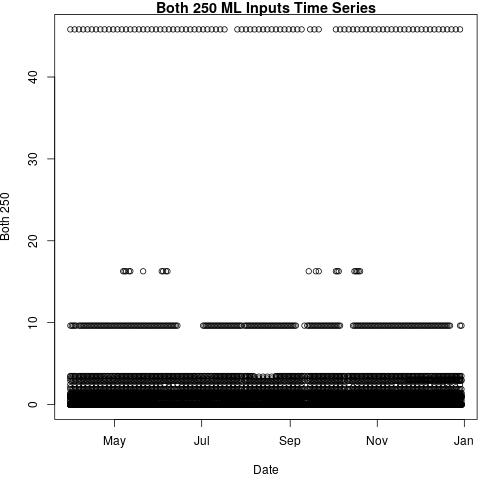
\includegraphics[width=0.77\textwidth]{Code_Outputs/Report_ML_input_PM25_Step4_part_e_de_duplicated_aves_Both_250vDate.jpg} 
\caption{\label{fig:Report_ML_input_PM25_Step4_part_e_de_duplicated_avesBoth_250vDate}ML Inputs Time Series} 
\end{figure} 
 

\begin{figure} 
\centering  
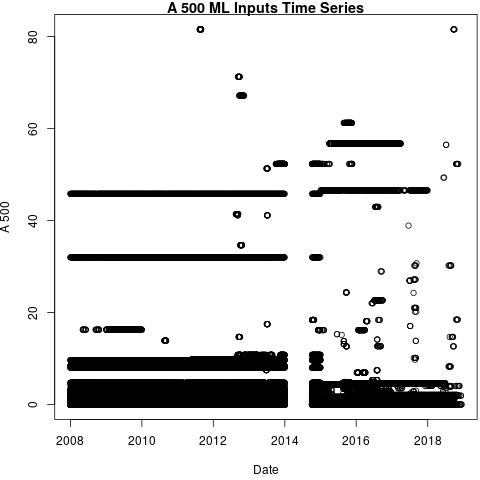
\includegraphics[width=0.77\textwidth]{Code_Outputs/Report_ML_input_PM25_Step4_part_e_de_duplicated_aves_A_500vDate.jpg} 
\caption{\label{fig:Report_ML_input_PM25_Step4_part_e_de_duplicated_avesA_500vDate}ML Inputs Time Series} 
\end{figure} 
 

\begin{figure} 
\centering  
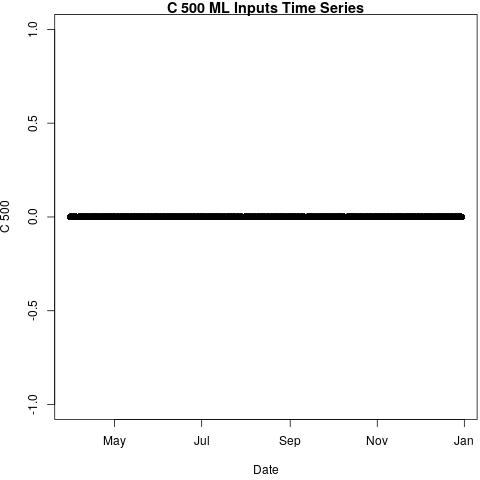
\includegraphics[width=0.77\textwidth]{Code_Outputs/Report_ML_input_PM25_Step4_part_e_de_duplicated_aves_C_500vDate.jpg} 
\caption{\label{fig:Report_ML_input_PM25_Step4_part_e_de_duplicated_avesC_500vDate}ML Inputs Time Series} 
\end{figure} 
 

\begin{figure} 
\centering  
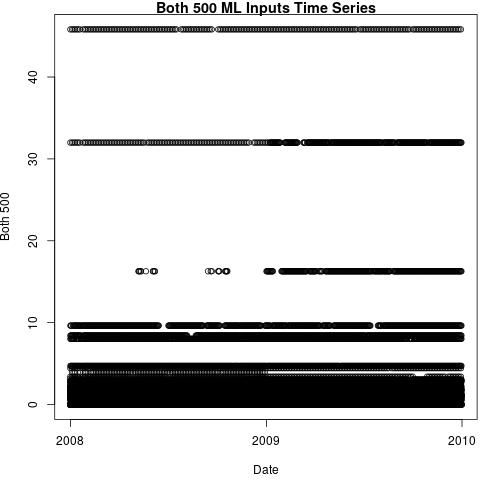
\includegraphics[width=0.77\textwidth]{Code_Outputs/Report_ML_input_PM25_Step4_part_e_de_duplicated_aves_Both_500vDate.jpg} 
\caption{\label{fig:Report_ML_input_PM25_Step4_part_e_de_duplicated_avesBoth_500vDate}ML Inputs Time Series} 
\end{figure} 
 

\begin{figure} 
\centering  
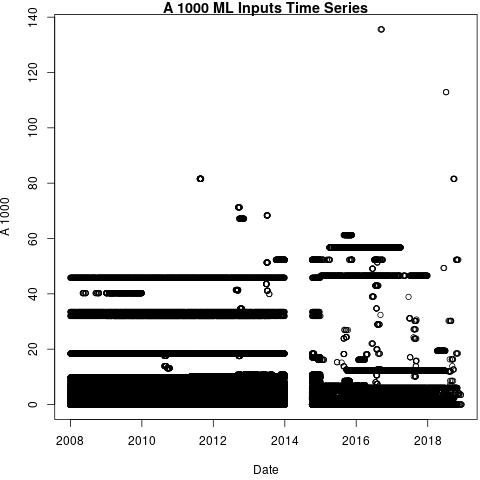
\includegraphics[width=0.77\textwidth]{Code_Outputs/Report_ML_input_PM25_Step4_part_e_de_duplicated_aves_A_1000vDate.jpg} 
\caption{\label{fig:Report_ML_input_PM25_Step4_part_e_de_duplicated_avesA_1000vDate}ML Inputs Time Series} 
\end{figure} 
 

\begin{figure} 
\centering  
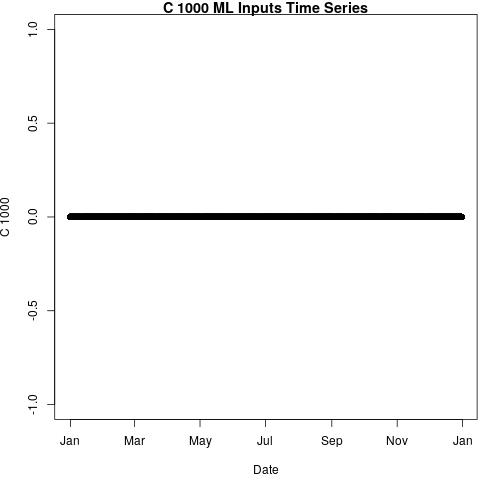
\includegraphics[width=0.77\textwidth]{Code_Outputs/Report_ML_input_PM25_Step4_part_e_de_duplicated_aves_C_1000vDate.jpg} 
\caption{\label{fig:Report_ML_input_PM25_Step4_part_e_de_duplicated_avesC_1000vDate}ML Inputs Time Series} 
\end{figure} 
 

\begin{figure} 
\centering  
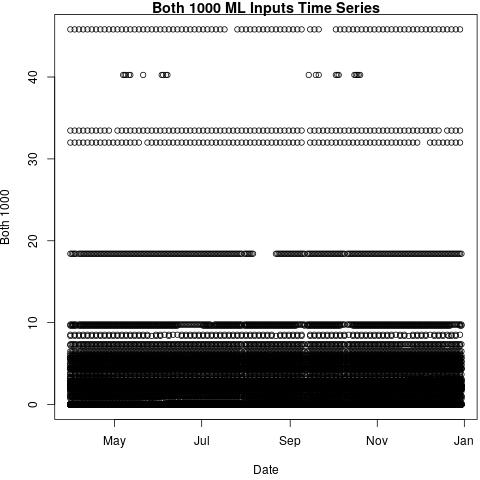
\includegraphics[width=0.77\textwidth]{Code_Outputs/Report_ML_input_PM25_Step4_part_e_de_duplicated_aves_Both_1000vDate.jpg} 
\caption{\label{fig:Report_ML_input_PM25_Step4_part_e_de_duplicated_avesBoth_1000vDate}ML Inputs Time Series} 
\end{figure} 
 

\begin{figure} 
\centering  
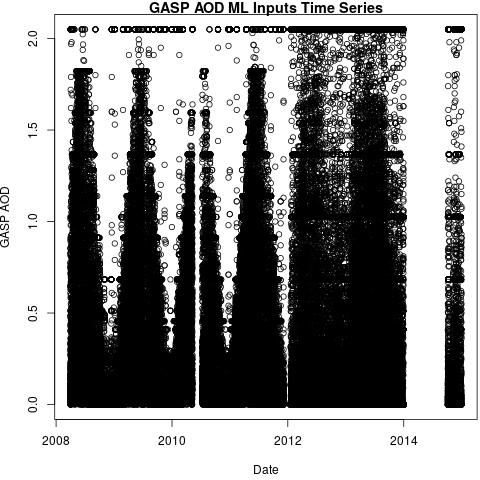
\includegraphics[width=0.77\textwidth]{Code_Outputs/Report_ML_input_PM25_Step4_part_e_de_duplicated_aves_GASP_AODvDate.jpg} 
\caption{\label{fig:Report_ML_input_PM25_Step4_part_e_de_duplicated_avesGASP_AODvDate}ML Inputs Time Series} 
\end{figure} 
 

\begin{figure} 
\centering  
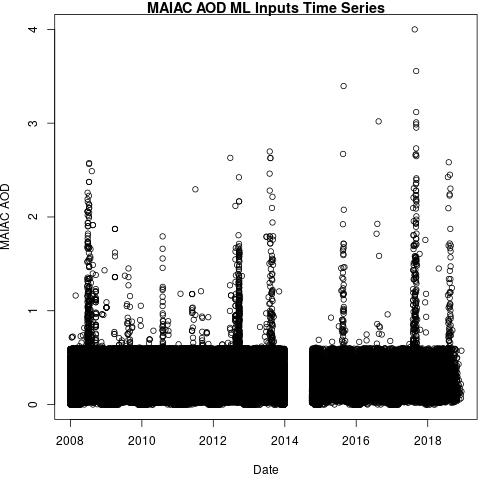
\includegraphics[width=0.77\textwidth]{Code_Outputs/Report_ML_input_PM25_Step4_part_e_de_duplicated_aves_MAIAC_AODvDate.jpg} 
\caption{\label{fig:Report_ML_input_PM25_Step4_part_e_de_duplicated_avesMAIAC_AODvDate}ML Inputs Time Series} 
\end{figure} 
 

\begin{figure} 
\centering  
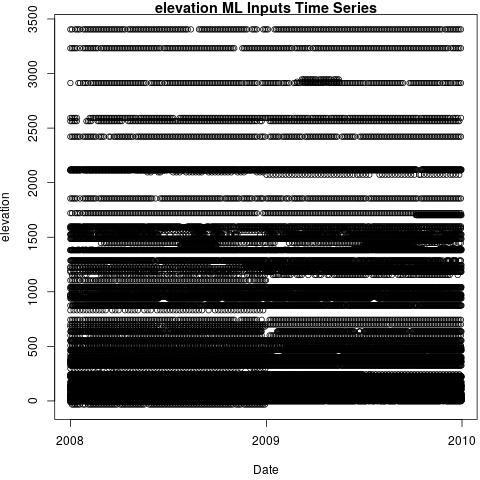
\includegraphics[width=0.77\textwidth]{Code_Outputs/Report_ML_input_PM25_Step4_part_e_de_duplicated_aves_elevationvDate.jpg} 
\caption{\label{fig:Report_ML_input_PM25_Step4_part_e_de_duplicated_aveselevationvDate}ML Inputs Time Series} 
\end{figure} 
 

\clearpage 

\begin{figure} 
\centering  
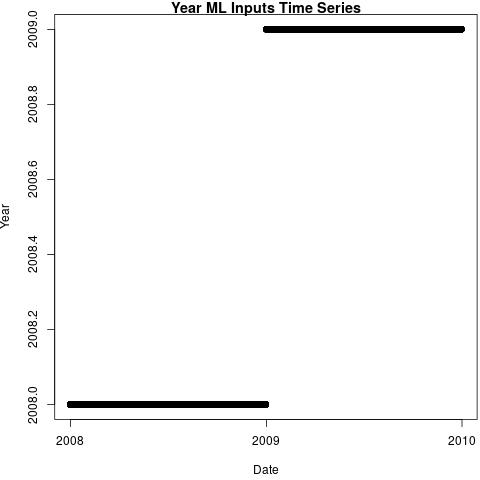
\includegraphics[width=0.77\textwidth]{Code_Outputs/Report_ML_input_PM25_Step4_part_e_de_duplicated_aves_YearvDate.jpg} 
\caption{\label{fig:Report_ML_input_PM25_Step4_part_e_de_duplicated_avesYearvDate}ML Inputs Time Series} 
\end{figure} 
 

\begin{figure} 
\centering  
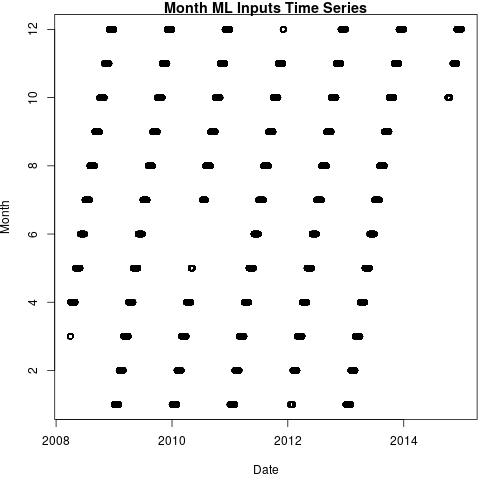
\includegraphics[width=0.77\textwidth]{Code_Outputs/Report_ML_input_PM25_Step4_part_e_de_duplicated_aves_MonthvDate.jpg} 
\caption{\label{fig:Report_ML_input_PM25_Step4_part_e_de_duplicated_avesMonthvDate}ML Inputs Time Series} 
\end{figure} 
 

\begin{figure} 
\centering  
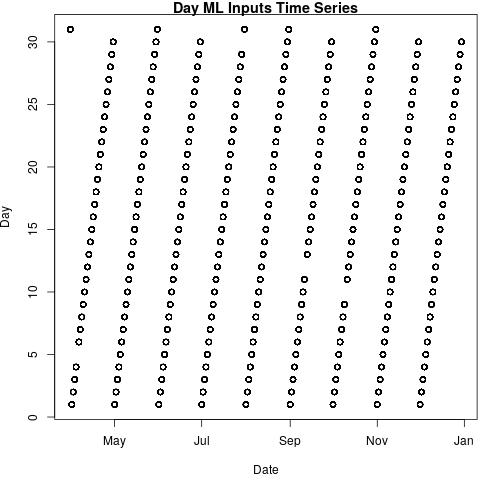
\includegraphics[width=0.77\textwidth]{Code_Outputs/Report_ML_input_PM25_Step4_part_e_de_duplicated_aves_DayvDate.jpg} 
\caption{\label{fig:Report_ML_input_PM25_Step4_part_e_de_duplicated_avesDayvDate}ML Inputs Time Series} 
\end{figure} 
 

\begin{figure} 
\centering  
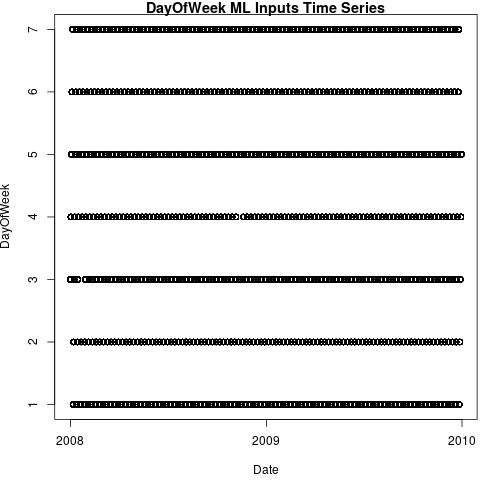
\includegraphics[width=0.77\textwidth]{Code_Outputs/Report_ML_input_PM25_Step4_part_e_de_duplicated_aves_DayOfWeekvDate.jpg} 
\caption{\label{fig:Report_ML_input_PM25_Step4_part_e_de_duplicated_avesDayOfWeekvDate}ML Inputs Time Series} 
\end{figure} 
 

\begin{figure} 
\centering  
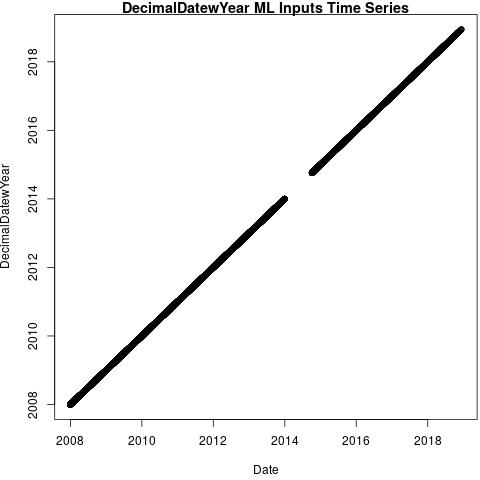
\includegraphics[width=0.77\textwidth]{Code_Outputs/Report_ML_input_PM25_Step4_part_e_de_duplicated_aves_DecimalDatewYearvDate.jpg} 
\caption{\label{fig:Report_ML_input_PM25_Step4_part_e_de_duplicated_avesDecimalDatewYearvDate}ML Inputs Time Series} 
\end{figure} 
 

\begin{figure} 
\centering  
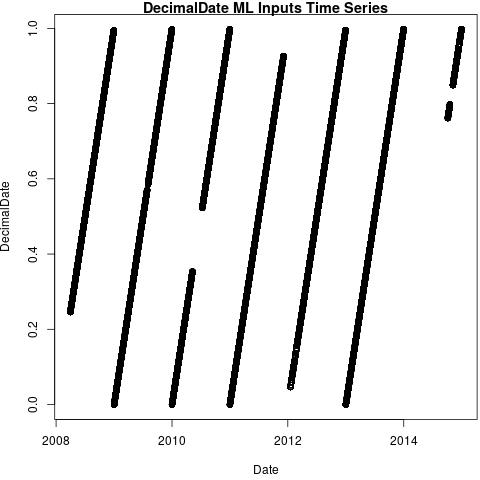
\includegraphics[width=0.77\textwidth]{Code_Outputs/Report_ML_input_PM25_Step4_part_e_de_duplicated_aves_DecimalDatevDate.jpg} 
\caption{\label{fig:Report_ML_input_PM25_Step4_part_e_de_duplicated_avesDecimalDatevDate}ML Inputs Time Series} 
\end{figure} 
 
 

% PM2.5 vs predictor for each predictor variable

\subsection{ML Inputs Plot against PM2.5 Images} 
 

\begin{figure} 
\centering  
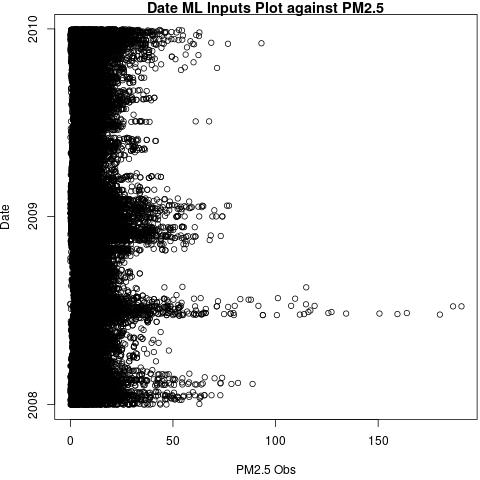
\includegraphics[width=0.77\textwidth]{Code_Outputs/Report_ML_input_PM25_Step4_part_e_de_duplicated_aves_DatevPM25_Obs.jpg} 
\caption{\label{fig:Report_ML_input_PM25_Step4_part_e_de_duplicated_avesDatevPM25_Obs}ML Inputs Plot against PM2.5} 
\end{figure} 
 

\begin{figure} 
\centering  
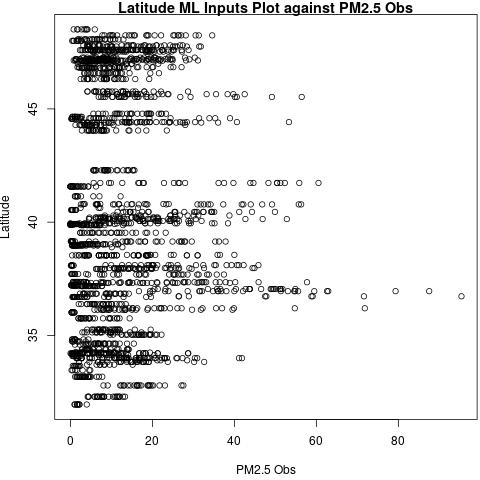
\includegraphics[width=0.77\textwidth]{Code_Outputs/Report_ML_input_PM25_Step4_part_e_de_duplicated_aves_LatitudevPM25_Obs.jpg} 
\caption{\label{fig:Report_ML_input_PM25_Step4_part_e_de_duplicated_avesLatitudevPM25_Obs}ML Inputs Plot against PM2.5} 
\end{figure} 
 

\begin{figure} 
\centering  
\includegraphics[width=0.77\textwidth]{Code_Outputs/Report_ML_input_PM25_Step4_part_e_de_duplicated_aves_LongitudevPM25_Obs.jpg} 
\caption{\label{fig:Report_ML_input_PM25_Step4_part_e_de_duplicated_avesLongitudevPM25_Obs}ML Inputs Plot against PM2.5} 
\end{figure} 
 

\begin{figure} 
\centering  
\includegraphics[width=0.77\textwidth]{Code_Outputs/Report_ML_input_PM25_Step4_part_e_de_duplicated_aves_A_100vPM25_Obs.jpg} 
\caption{\label{fig:Report_ML_input_PM25_Step4_part_e_de_duplicated_avesA_100vPM25_Obs}ML Inputs Plot against PM2.5} 
\end{figure} 
 

\begin{figure} 
\centering  
\includegraphics[width=0.77\textwidth]{Code_Outputs/Report_ML_input_PM25_Step4_part_e_de_duplicated_aves_C_100vPM25_Obs.jpg} 
\caption{\label{fig:Report_ML_input_PM25_Step4_part_e_de_duplicated_avesC_100vPM25_Obs}ML Inputs Plot against PM2.5} 
\end{figure} 
 

\begin{figure} 
\centering  
\includegraphics[width=0.77\textwidth]{Code_Outputs/Report_ML_input_PM25_Step4_part_e_de_duplicated_aves_Both_100vPM25_Obs.jpg} 
\caption{\label{fig:Report_ML_input_PM25_Step4_part_e_de_duplicated_avesBoth_100vPM25_Obs}ML Inputs Plot against PM2.5} 
\end{figure} 
 

\begin{figure} 
\centering  
\includegraphics[width=0.77\textwidth]{Code_Outputs/Report_ML_input_PM25_Step4_part_e_de_duplicated_aves_A_250vPM25_Obs.jpg} 
\caption{\label{fig:Report_ML_input_PM25_Step4_part_e_de_duplicated_avesA_250vPM25_Obs}ML Inputs Plot against PM2.5} 
\end{figure} 
 

\begin{figure} 
\centering  
\includegraphics[width=0.77\textwidth]{Code_Outputs/Report_ML_input_PM25_Step4_part_e_de_duplicated_aves_C_250vPM25_Obs.jpg} 
\caption{\label{fig:Report_ML_input_PM25_Step4_part_e_de_duplicated_avesC_250vPM25_Obs}ML Inputs Plot against PM2.5} 
\end{figure} 
 

\begin{figure} 
\centering  
\includegraphics[width=0.77\textwidth]{Code_Outputs/Report_ML_input_PM25_Step4_part_e_de_duplicated_aves_Both_250vPM25_Obs.jpg} 
\caption{\label{fig:Report_ML_input_PM25_Step4_part_e_de_duplicated_avesBoth_250vPM25_Obs}ML Inputs Plot against PM2.5} 
\end{figure} 
 

\clearpage 

\begin{figure} 
\centering  
\includegraphics[width=0.77\textwidth]{Code_Outputs/Report_ML_input_PM25_Step4_part_e_de_duplicated_aves_A_500vPM25_Obs.jpg} 
\caption{\label{fig:Report_ML_input_PM25_Step4_part_e_de_duplicated_avesA_500vPM25_Obs}ML Inputs Plot against PM2.5} 
\end{figure} 
 

\begin{figure} 
\centering  
\includegraphics[width=0.77\textwidth]{Code_Outputs/Report_ML_input_PM25_Step4_part_e_de_duplicated_aves_C_500vPM25_Obs.jpg} 
\caption{\label{fig:Report_ML_input_PM25_Step4_part_e_de_duplicated_avesC_500vPM25_Obs}ML Inputs Plot against PM2.5} 
\end{figure} 
 

\begin{figure} 
\centering  
\includegraphics[width=0.77\textwidth]{Code_Outputs/Report_ML_input_PM25_Step4_part_e_de_duplicated_aves_Both_500vPM25_Obs.jpg} 
\caption{\label{fig:Report_ML_input_PM25_Step4_part_e_de_duplicated_avesBoth_500vPM25_Obs}ML Inputs Plot against PM2.5} 
\end{figure} 
 

\begin{figure} 
\centering  
\includegraphics[width=0.77\textwidth]{Code_Outputs/Report_ML_input_PM25_Step4_part_e_de_duplicated_aves_A_1000vPM25_Obs.jpg} 
\caption{\label{fig:Report_ML_input_PM25_Step4_part_e_de_duplicated_avesA_1000vPM25_Obs}ML Inputs Plot against PM2.5} 
\end{figure} 
 

\begin{figure} 
\centering  
\includegraphics[width=0.77\textwidth]{Code_Outputs/Report_ML_input_PM25_Step4_part_e_de_duplicated_aves_C_1000vPM25_Obs.jpg} 
\caption{\label{fig:Report_ML_input_PM25_Step4_part_e_de_duplicated_avesC_1000vPM25_Obs}ML Inputs Plot against PM2.5} 
\end{figure} 
 

\begin{figure} 
\centering  
\includegraphics[width=0.77\textwidth]{Code_Outputs/Report_ML_input_PM25_Step4_part_e_de_duplicated_aves_Both_1000vPM25_Obs.jpg} 
\caption{\label{fig:Report_ML_input_PM25_Step4_part_e_de_duplicated_avesBoth_1000vPM25_Obs}ML Inputs Plot against PM2.5} 
\end{figure} 
 

\begin{figure} 
\centering  
\includegraphics[width=0.77\textwidth]{Code_Outputs/Report_ML_input_PM25_Step4_part_e_de_duplicated_aves_YearvPM25_Obs.jpg} 
\caption{\label{fig:Report_ML_input_PM25_Step4_part_e_de_duplicated_avesYearvPM25_Obs}ML Inputs Plot against PM2.5} 
\end{figure} 
 

\begin{figure} 
\centering  
\includegraphics[width=0.77\textwidth]{Code_Outputs/Report_ML_input_PM25_Step4_part_e_de_duplicated_aves_MonthvPM25_Obs.jpg} 
\caption{\label{fig:Report_ML_input_PM25_Step4_part_e_de_duplicated_avesMonthvPM25_Obs}ML Inputs Plot against PM2.5} 
\end{figure} 
 

\begin{figure} 
\centering  
\includegraphics[width=0.77\textwidth]{Code_Outputs/Report_ML_input_PM25_Step4_part_e_de_duplicated_aves_DayvPM25_Obs.jpg} 
\caption{\label{fig:Report_ML_input_PM25_Step4_part_e_de_duplicated_avesDayvPM25_Obs}ML Inputs Plot against PM2.5} 
\end{figure} 
 

\begin{figure} 
\centering  
\includegraphics[width=0.77\textwidth]{Code_Outputs/Report_ML_input_PM25_Step4_part_e_de_duplicated_aves_DayOfWeekvPM25_Obs.jpg} 
\caption{\label{fig:Report_ML_input_PM25_Step4_part_e_de_duplicated_avesDayOfWeekvPM25_Obs}ML Inputs Plot against PM2.5} 
\end{figure} 
 

\clearpage 

\begin{figure} 
\centering  
\includegraphics[width=0.77\textwidth]{Code_Outputs/Report_ML_input_PM25_Step4_part_e_de_duplicated_aves_DecimalDatewYearvPM25_Obs.jpg} 
\caption{\label{fig:Report_ML_input_PM25_Step4_part_e_de_duplicated_avesDecimalDatewYearvPM25_Obs}ML Inputs Plot against PM2.5} 
\end{figure} 
 

\begin{figure} 
\centering  
\includegraphics[width=0.77\textwidth]{Code_Outputs/Report_ML_input_PM25_Step4_part_e_de_duplicated_aves_DecimalDatevPM25_Obs.jpg} 
\caption{\label{fig:Report_ML_input_PM25_Step4_part_e_de_duplicated_avesDecimalDatevPM25_Obs}ML Inputs Plot against PM2.5} 
\end{figure} 
 
 

% plot maps of a few specific days

\subsection{ML Inputs Map subset of days Images} 
 

\begin{figure} 
\centering  
\includegraphics[width=0.77\textwidth]{Code_Outputs/Report_ML_input_PM25_Step4_part_e_de_duplicated_aves_MapObsPM25_Obs2008-07-10.jpg} 
\caption{\label{fig:Report_ML_input_PM25_Step4_part_e_de_duplicated_avesMapObsPM25_Obs2008-07-10}PM2.5 Obs 2008-07-10} 
\end{figure} 
 

\begin{figure} 
\centering  
\includegraphics[width=0.77\textwidth]{Code_Outputs/Report_ML_input_PM25_Step4_part_e_de_duplicated_aves_MapObsPM25_Obs2008-06-24.jpg} 
\caption{\label{fig:Report_ML_input_PM25_Step4_part_e_de_duplicated_avesMapObsPM25_Obs2008-06-24}PM2.5 Obs 2008-06-24} 
\end{figure} 
 

\begin{figure} 
\centering  
\includegraphics[width=0.77\textwidth]{Code_Outputs/Report_ML_input_PM25_Step4_part_e_de_duplicated_aves_MapObsPM25_Obs2008-06-27.jpg} 
\caption{\label{fig:Report_ML_input_PM25_Step4_part_e_de_duplicated_avesMapObsPM25_Obs2008-06-27}PM2.5 Obs 2008-06-27} 
\end{figure} 
 

\begin{figure} 
\centering  
\includegraphics[width=0.77\textwidth]{Code_Outputs/Report_ML_input_PM25_Step4_part_e_de_duplicated_aves_MapObsPM25_Obs2009-03-22.jpg} 
\caption{\label{fig:Report_ML_input_PM25_Step4_part_e_de_duplicated_avesMapObsPM25_Obs2009-03-22}PM2.5 Obs 2009-03-22} 
\end{figure} 
 

\begin{figure} 
\centering  
\includegraphics[width=0.77\textwidth]{Code_Outputs/Report_ML_input_PM25_Step4_part_e_de_duplicated_aves_MapObsPM25_Obs2009-06-07.jpg} 
\caption{\label{fig:Report_ML_input_PM25_Step4_part_e_de_duplicated_avesMapObsPM25_Obs2009-06-07}PM2.5 Obs 2009-06-07} 
\end{figure} 
 

\begin{figure} 
\centering  
\includegraphics[width=0.77\textwidth]{Code_Outputs/Report_ML_input_PM25_Step4_part_e_de_duplicated_aves_MapObsPM25_Obs2009-04-15.jpg} 
\caption{\label{fig:Report_ML_input_PM25_Step4_part_e_de_duplicated_avesMapObsPM25_Obs2009-04-15}PM2.5 Obs 2009-04-15} 
\end{figure} 
 

\begin{figure} 
\centering  
\includegraphics[width=0.77\textwidth]{Code_Outputs/Report_ML_input_PM25_Step4_part_e_de_duplicated_aves_MapObsA_1002008-07-10.jpg} 
\caption{\label{fig:Report_ML_input_PM25_Step4_part_e_de_duplicated_avesMapObsA_1002008-07-10}A 100 2008-07-10} 
\end{figure} 
 

\begin{figure} 
\centering  
\includegraphics[width=0.77\textwidth]{Code_Outputs/Report_ML_input_PM25_Step4_part_e_de_duplicated_aves_MapObsA_1002008-06-24.jpg} 
\caption{\label{fig:Report_ML_input_PM25_Step4_part_e_de_duplicated_avesMapObsA_1002008-06-24}A 100 2008-06-24} 
\end{figure} 
 

\begin{figure} 
\centering  
\includegraphics[width=0.77\textwidth]{Code_Outputs/Report_ML_input_PM25_Step4_part_e_de_duplicated_aves_MapObsA_1002008-06-27.jpg} 
\caption{\label{fig:Report_ML_input_PM25_Step4_part_e_de_duplicated_avesMapObsA_1002008-06-27}A 100 2008-06-27} 
\end{figure} 
 

\clearpage 

\begin{figure} 
\centering  
\includegraphics[width=0.77\textwidth]{Code_Outputs/Report_ML_input_PM25_Step4_part_e_de_duplicated_aves_MapObsA_1002009-03-22.jpg} 
\caption{\label{fig:Report_ML_input_PM25_Step4_part_e_de_duplicated_avesMapObsA_1002009-03-22}A 100 2009-03-22} 
\end{figure} 
 

\begin{figure} 
\centering  
\includegraphics[width=0.77\textwidth]{Code_Outputs/Report_ML_input_PM25_Step4_part_e_de_duplicated_aves_MapObsA_1002009-06-07.jpg} 
\caption{\label{fig:Report_ML_input_PM25_Step4_part_e_de_duplicated_avesMapObsA_1002009-06-07}A 100 2009-06-07} 
\end{figure} 
 

\begin{figure} 
\centering  
\includegraphics[width=0.77\textwidth]{Code_Outputs/Report_ML_input_PM25_Step4_part_e_de_duplicated_aves_MapObsA_1002009-04-15.jpg} 
\caption{\label{fig:Report_ML_input_PM25_Step4_part_e_de_duplicated_avesMapObsA_1002009-04-15}A 100 2009-04-15} 
\end{figure} 
 

\begin{figure} 
\centering  
\includegraphics[width=0.77\textwidth]{Code_Outputs/Report_ML_input_PM25_Step4_part_e_de_duplicated_aves_MapObsC_1002008-07-10.jpg} 
\caption{\label{fig:Report_ML_input_PM25_Step4_part_e_de_duplicated_avesMapObsC_1002008-07-10}C 100 2008-07-10} 
\end{figure} 
 

\begin{figure} 
\centering  
\includegraphics[width=0.77\textwidth]{Code_Outputs/Report_ML_input_PM25_Step4_part_e_de_duplicated_aves_MapObsC_1002008-06-24.jpg} 
\caption{\label{fig:Report_ML_input_PM25_Step4_part_e_de_duplicated_avesMapObsC_1002008-06-24}C 100 2008-06-24} 
\end{figure} 
 

\begin{figure} 
\centering  
\includegraphics[width=0.77\textwidth]{Code_Outputs/Report_ML_input_PM25_Step4_part_e_de_duplicated_aves_MapObsC_1002008-06-27.jpg} 
\caption{\label{fig:Report_ML_input_PM25_Step4_part_e_de_duplicated_avesMapObsC_1002008-06-27}C 100 2008-06-27} 
\end{figure} 
 

\begin{figure} 
\centering  
\includegraphics[width=0.77\textwidth]{Code_Outputs/Report_ML_input_PM25_Step4_part_e_de_duplicated_aves_MapObsC_1002009-03-22.jpg} 
\caption{\label{fig:Report_ML_input_PM25_Step4_part_e_de_duplicated_avesMapObsC_1002009-03-22}C 100 2009-03-22} 
\end{figure} 
 

\begin{figure} 
\centering  
\includegraphics[width=0.77\textwidth]{Code_Outputs/Report_ML_input_PM25_Step4_part_e_de_duplicated_aves_MapObsC_1002009-06-07.jpg} 
\caption{\label{fig:Report_ML_input_PM25_Step4_part_e_de_duplicated_avesMapObsC_1002009-06-07}C 100 2009-06-07} 
\end{figure} 
 

\begin{figure} 
\centering  
\includegraphics[width=0.77\textwidth]{Code_Outputs/Report_ML_input_PM25_Step4_part_e_de_duplicated_aves_MapObsC_1002009-04-15.jpg} 
\caption{\label{fig:Report_ML_input_PM25_Step4_part_e_de_duplicated_avesMapObsC_1002009-04-15}C 100 2009-04-15} 
\end{figure} 
 

\begin{figure} 
\centering  
\includegraphics[width=0.77\textwidth]{Code_Outputs/Report_ML_input_PM25_Step4_part_e_de_duplicated_aves_MapObsBoth_1002008-07-10.jpg} 
\caption{\label{fig:Report_ML_input_PM25_Step4_part_e_de_duplicated_avesMapObsBoth_1002008-07-10}Both 100 2008-07-10} 
\end{figure} 
 

\clearpage 

\begin{figure} 
\centering  
\includegraphics[width=0.77\textwidth]{Code_Outputs/Report_ML_input_PM25_Step4_part_e_de_duplicated_aves_MapObsBoth_1002008-06-24.jpg} 
\caption{\label{fig:Report_ML_input_PM25_Step4_part_e_de_duplicated_avesMapObsBoth_1002008-06-24}Both 100 2008-06-24} 
\end{figure} 
 

\begin{figure} 
\centering  
\includegraphics[width=0.77\textwidth]{Code_Outputs/Report_ML_input_PM25_Step4_part_e_de_duplicated_aves_MapObsBoth_1002008-06-27.jpg} 
\caption{\label{fig:Report_ML_input_PM25_Step4_part_e_de_duplicated_avesMapObsBoth_1002008-06-27}Both 100 2008-06-27} 
\end{figure} 
 

\begin{figure} 
\centering  
\includegraphics[width=0.77\textwidth]{Code_Outputs/Report_ML_input_PM25_Step4_part_e_de_duplicated_aves_MapObsBoth_1002009-03-22.jpg} 
\caption{\label{fig:Report_ML_input_PM25_Step4_part_e_de_duplicated_avesMapObsBoth_1002009-03-22}Both 100 2009-03-22} 
\end{figure} 
 

\begin{figure} 
\centering  
\includegraphics[width=0.77\textwidth]{Code_Outputs/Report_ML_input_PM25_Step4_part_e_de_duplicated_aves_MapObsBoth_1002009-06-07.jpg} 
\caption{\label{fig:Report_ML_input_PM25_Step4_part_e_de_duplicated_avesMapObsBoth_1002009-06-07}Both 100 2009-06-07} 
\end{figure} 
 

\begin{figure} 
\centering  
\includegraphics[width=0.77\textwidth]{Code_Outputs/Report_ML_input_PM25_Step4_part_e_de_duplicated_aves_MapObsBoth_1002009-04-15.jpg} 
\caption{\label{fig:Report_ML_input_PM25_Step4_part_e_de_duplicated_avesMapObsBoth_1002009-04-15}Both 100 2009-04-15} 
\end{figure} 
 

\begin{figure} 
\centering  
\includegraphics[width=0.77\textwidth]{Code_Outputs/Report_ML_input_PM25_Step4_part_e_de_duplicated_aves_MapObsA_2502008-07-10.jpg} 
\caption{\label{fig:Report_ML_input_PM25_Step4_part_e_de_duplicated_avesMapObsA_2502008-07-10}A 250 2008-07-10} 
\end{figure} 
 

\begin{figure} 
\centering  
\includegraphics[width=0.77\textwidth]{Code_Outputs/Report_ML_input_PM25_Step4_part_e_de_duplicated_aves_MapObsA_2502008-06-24.jpg} 
\caption{\label{fig:Report_ML_input_PM25_Step4_part_e_de_duplicated_avesMapObsA_2502008-06-24}A 250 2008-06-24} 
\end{figure} 
 

\begin{figure} 
\centering  
\includegraphics[width=0.77\textwidth]{Code_Outputs/Report_ML_input_PM25_Step4_part_e_de_duplicated_aves_MapObsA_2502008-06-27.jpg} 
\caption{\label{fig:Report_ML_input_PM25_Step4_part_e_de_duplicated_avesMapObsA_2502008-06-27}A 250 2008-06-27} 
\end{figure} 
 

\begin{figure} 
\centering  
\includegraphics[width=0.77\textwidth]{Code_Outputs/Report_ML_input_PM25_Step4_part_e_de_duplicated_aves_MapObsA_2502009-03-22.jpg} 
\caption{\label{fig:Report_ML_input_PM25_Step4_part_e_de_duplicated_avesMapObsA_2502009-03-22}A 250 2009-03-22} 
\end{figure} 
 

\begin{figure} 
\centering  
\includegraphics[width=0.77\textwidth]{Code_Outputs/Report_ML_input_PM25_Step4_part_e_de_duplicated_aves_MapObsA_2502009-06-07.jpg} 
\caption{\label{fig:Report_ML_input_PM25_Step4_part_e_de_duplicated_avesMapObsA_2502009-06-07}A 250 2009-06-07} 
\end{figure} 
 

\clearpage 

\begin{figure} 
\centering  
\includegraphics[width=0.77\textwidth]{Code_Outputs/Report_ML_input_PM25_Step4_part_e_de_duplicated_aves_MapObsA_2502009-04-15.jpg} 
\caption{\label{fig:Report_ML_input_PM25_Step4_part_e_de_duplicated_avesMapObsA_2502009-04-15}A 250 2009-04-15} 
\end{figure} 
 

\begin{figure} 
\centering  
\includegraphics[width=0.77\textwidth]{Code_Outputs/Report_ML_input_PM25_Step4_part_e_de_duplicated_aves_MapObsC_2502008-07-10.jpg} 
\caption{\label{fig:Report_ML_input_PM25_Step4_part_e_de_duplicated_avesMapObsC_2502008-07-10}C 250 2008-07-10} 
\end{figure} 
 

\begin{figure} 
\centering  
\includegraphics[width=0.77\textwidth]{Code_Outputs/Report_ML_input_PM25_Step4_part_e_de_duplicated_aves_MapObsC_2502008-06-24.jpg} 
\caption{\label{fig:Report_ML_input_PM25_Step4_part_e_de_duplicated_avesMapObsC_2502008-06-24}C 250 2008-06-24} 
\end{figure} 
 

\begin{figure} 
\centering  
\includegraphics[width=0.77\textwidth]{Code_Outputs/Report_ML_input_PM25_Step4_part_e_de_duplicated_aves_MapObsC_2502008-06-27.jpg} 
\caption{\label{fig:Report_ML_input_PM25_Step4_part_e_de_duplicated_avesMapObsC_2502008-06-27}C 250 2008-06-27} 
\end{figure} 
 

\begin{figure} 
\centering  
\includegraphics[width=0.77\textwidth]{Code_Outputs/Report_ML_input_PM25_Step4_part_e_de_duplicated_aves_MapObsC_2502009-03-22.jpg} 
\caption{\label{fig:Report_ML_input_PM25_Step4_part_e_de_duplicated_avesMapObsC_2502009-03-22}C 250 2009-03-22} 
\end{figure} 
 

\begin{figure} 
\centering  
\includegraphics[width=0.77\textwidth]{Code_Outputs/Report_ML_input_PM25_Step4_part_e_de_duplicated_aves_MapObsC_2502009-06-07.jpg} 
\caption{\label{fig:Report_ML_input_PM25_Step4_part_e_de_duplicated_avesMapObsC_2502009-06-07}C 250 2009-06-07} 
\end{figure} 
 

\begin{figure} 
\centering  
\includegraphics[width=0.77\textwidth]{Code_Outputs/Report_ML_input_PM25_Step4_part_e_de_duplicated_aves_MapObsC_2502009-04-15.jpg} 
\caption{\label{fig:Report_ML_input_PM25_Step4_part_e_de_duplicated_avesMapObsC_2502009-04-15}C 250 2009-04-15} 
\end{figure} 
 

\begin{figure} 
\centering  
\includegraphics[width=0.77\textwidth]{Code_Outputs/Report_ML_input_PM25_Step4_part_e_de_duplicated_aves_MapObsBoth_2502008-07-10.jpg} 
\caption{\label{fig:Report_ML_input_PM25_Step4_part_e_de_duplicated_avesMapObsBoth_2502008-07-10}Both 250 2008-07-10} 
\end{figure} 
 

\begin{figure} 
\centering  
\includegraphics[width=0.77\textwidth]{Code_Outputs/Report_ML_input_PM25_Step4_part_e_de_duplicated_aves_MapObsBoth_2502008-06-24.jpg} 
\caption{\label{fig:Report_ML_input_PM25_Step4_part_e_de_duplicated_avesMapObsBoth_2502008-06-24}Both 250 2008-06-24} 
\end{figure} 
 

\begin{figure} 
\centering  
\includegraphics[width=0.77\textwidth]{Code_Outputs/Report_ML_input_PM25_Step4_part_e_de_duplicated_aves_MapObsBoth_2502008-06-27.jpg} 
\caption{\label{fig:Report_ML_input_PM25_Step4_part_e_de_duplicated_avesMapObsBoth_2502008-06-27}Both 250 2008-06-27} 
\end{figure} 
 

\clearpage 

\begin{figure} 
\centering  
\includegraphics[width=0.77\textwidth]{Code_Outputs/Report_ML_input_PM25_Step4_part_e_de_duplicated_aves_MapObsBoth_2502009-03-22.jpg} 
\caption{\label{fig:Report_ML_input_PM25_Step4_part_e_de_duplicated_avesMapObsBoth_2502009-03-22}Both 250 2009-03-22} 
\end{figure} 
 

\begin{figure} 
\centering  
\includegraphics[width=0.77\textwidth]{Code_Outputs/Report_ML_input_PM25_Step4_part_e_de_duplicated_aves_MapObsBoth_2502009-06-07.jpg} 
\caption{\label{fig:Report_ML_input_PM25_Step4_part_e_de_duplicated_avesMapObsBoth_2502009-06-07}Both 250 2009-06-07} 
\end{figure} 
 

\begin{figure} 
\centering  
\includegraphics[width=0.77\textwidth]{Code_Outputs/Report_ML_input_PM25_Step4_part_e_de_duplicated_aves_MapObsBoth_2502009-04-15.jpg} 
\caption{\label{fig:Report_ML_input_PM25_Step4_part_e_de_duplicated_avesMapObsBoth_2502009-04-15}Both 250 2009-04-15} 
\end{figure} 
 

\begin{figure} 
\centering  
\includegraphics[width=0.77\textwidth]{Code_Outputs/Report_ML_input_PM25_Step4_part_e_de_duplicated_aves_MapObsA_5002008-07-10.jpg} 
\caption{\label{fig:Report_ML_input_PM25_Step4_part_e_de_duplicated_avesMapObsA_5002008-07-10}A 500 2008-07-10} 
\end{figure} 
 

\begin{figure} 
\centering  
\includegraphics[width=0.77\textwidth]{Code_Outputs/Report_ML_input_PM25_Step4_part_e_de_duplicated_aves_MapObsA_5002008-06-24.jpg} 
\caption{\label{fig:Report_ML_input_PM25_Step4_part_e_de_duplicated_avesMapObsA_5002008-06-24}A 500 2008-06-24} 
\end{figure} 
 

\begin{figure} 
\centering  
\includegraphics[width=0.77\textwidth]{Code_Outputs/Report_ML_input_PM25_Step4_part_e_de_duplicated_aves_MapObsA_5002008-06-27.jpg} 
\caption{\label{fig:Report_ML_input_PM25_Step4_part_e_de_duplicated_avesMapObsA_5002008-06-27}A 500 2008-06-27} 
\end{figure} 
 

\begin{figure} 
\centering  
\includegraphics[width=0.77\textwidth]{Code_Outputs/Report_ML_input_PM25_Step4_part_e_de_duplicated_aves_MapObsA_5002009-03-22.jpg} 
\caption{\label{fig:Report_ML_input_PM25_Step4_part_e_de_duplicated_avesMapObsA_5002009-03-22}A 500 2009-03-22} 
\end{figure} 
 

\begin{figure} 
\centering  
\includegraphics[width=0.77\textwidth]{Code_Outputs/Report_ML_input_PM25_Step4_part_e_de_duplicated_aves_MapObsA_5002009-06-07.jpg} 
\caption{\label{fig:Report_ML_input_PM25_Step4_part_e_de_duplicated_avesMapObsA_5002009-06-07}A 500 2009-06-07} 
\end{figure} 
 

\begin{figure} 
\centering  
\includegraphics[width=0.77\textwidth]{Code_Outputs/Report_ML_input_PM25_Step4_part_e_de_duplicated_aves_MapObsA_5002009-04-15.jpg} 
\caption{\label{fig:Report_ML_input_PM25_Step4_part_e_de_duplicated_avesMapObsA_5002009-04-15}A 500 2009-04-15} 
\end{figure} 
 

\begin{figure} 
\centering  
\includegraphics[width=0.77\textwidth]{Code_Outputs/Report_ML_input_PM25_Step4_part_e_de_duplicated_aves_MapObsC_5002008-07-10.jpg} 
\caption{\label{fig:Report_ML_input_PM25_Step4_part_e_de_duplicated_avesMapObsC_5002008-07-10}C 500 2008-07-10} 
\end{figure} 
 

\clearpage 

\begin{figure} 
\centering  
\includegraphics[width=0.77\textwidth]{Code_Outputs/Report_ML_input_PM25_Step4_part_e_de_duplicated_aves_MapObsC_5002008-06-24.jpg} 
\caption{\label{fig:Report_ML_input_PM25_Step4_part_e_de_duplicated_avesMapObsC_5002008-06-24}C 500 2008-06-24} 
\end{figure} 
 

\begin{figure} 
\centering  
\includegraphics[width=0.77\textwidth]{Code_Outputs/Report_ML_input_PM25_Step4_part_e_de_duplicated_aves_MapObsC_5002008-06-27.jpg} 
\caption{\label{fig:Report_ML_input_PM25_Step4_part_e_de_duplicated_avesMapObsC_5002008-06-27}C 500 2008-06-27} 
\end{figure} 
 

\begin{figure} 
\centering  
\includegraphics[width=0.77\textwidth]{Code_Outputs/Report_ML_input_PM25_Step4_part_e_de_duplicated_aves_MapObsC_5002009-03-22.jpg} 
\caption{\label{fig:Report_ML_input_PM25_Step4_part_e_de_duplicated_avesMapObsC_5002009-03-22}C 500 2009-03-22} 
\end{figure} 
 

\begin{figure} 
\centering  
\includegraphics[width=0.77\textwidth]{Code_Outputs/Report_ML_input_PM25_Step4_part_e_de_duplicated_aves_MapObsC_5002009-06-07.jpg} 
\caption{\label{fig:Report_ML_input_PM25_Step4_part_e_de_duplicated_avesMapObsC_5002009-06-07}C 500 2009-06-07} 
\end{figure} 
 

\begin{figure} 
\centering  
\includegraphics[width=0.77\textwidth]{Code_Outputs/Report_ML_input_PM25_Step4_part_e_de_duplicated_aves_MapObsC_5002009-04-15.jpg} 
\caption{\label{fig:Report_ML_input_PM25_Step4_part_e_de_duplicated_avesMapObsC_5002009-04-15}C 500 2009-04-15} 
\end{figure} 
 

\begin{figure} 
\centering  
\includegraphics[width=0.77\textwidth]{Code_Outputs/Report_ML_input_PM25_Step4_part_e_de_duplicated_aves_MapObsBoth_5002008-07-10.jpg} 
\caption{\label{fig:Report_ML_input_PM25_Step4_part_e_de_duplicated_avesMapObsBoth_5002008-07-10}Both 500 2008-07-10} 
\end{figure} 
 

\begin{figure} 
\centering  
\includegraphics[width=0.77\textwidth]{Code_Outputs/Report_ML_input_PM25_Step4_part_e_de_duplicated_aves_MapObsBoth_5002008-06-24.jpg} 
\caption{\label{fig:Report_ML_input_PM25_Step4_part_e_de_duplicated_avesMapObsBoth_5002008-06-24}Both 500 2008-06-24} 
\end{figure} 
 

\begin{figure} 
\centering  
\includegraphics[width=0.77\textwidth]{Code_Outputs/Report_ML_input_PM25_Step4_part_e_de_duplicated_aves_MapObsBoth_5002008-06-27.jpg} 
\caption{\label{fig:Report_ML_input_PM25_Step4_part_e_de_duplicated_avesMapObsBoth_5002008-06-27}Both 500 2008-06-27} 
\end{figure} 
 

\begin{figure} 
\centering  
\includegraphics[width=0.77\textwidth]{Code_Outputs/Report_ML_input_PM25_Step4_part_e_de_duplicated_aves_MapObsBoth_5002009-03-22.jpg} 
\caption{\label{fig:Report_ML_input_PM25_Step4_part_e_de_duplicated_avesMapObsBoth_5002009-03-22}Both 500 2009-03-22} 
\end{figure} 
 

\begin{figure} 
\centering  
\includegraphics[width=0.77\textwidth]{Code_Outputs/Report_ML_input_PM25_Step4_part_e_de_duplicated_aves_MapObsBoth_5002009-06-07.jpg} 
\caption{\label{fig:Report_ML_input_PM25_Step4_part_e_de_duplicated_avesMapObsBoth_5002009-06-07}Both 500 2009-06-07} 
\end{figure} 
 

\clearpage 

\begin{figure} 
\centering  
\includegraphics[width=0.77\textwidth]{Code_Outputs/Report_ML_input_PM25_Step4_part_e_de_duplicated_aves_MapObsBoth_5002009-04-15.jpg} 
\caption{\label{fig:Report_ML_input_PM25_Step4_part_e_de_duplicated_avesMapObsBoth_5002009-04-15}Both 500 2009-04-15} 
\end{figure} 
 

\begin{figure} 
\centering  
\includegraphics[width=0.77\textwidth]{Code_Outputs/Report_ML_input_PM25_Step4_part_e_de_duplicated_aves_MapObsA_10002008-07-10.jpg} 
\caption{\label{fig:Report_ML_input_PM25_Step4_part_e_de_duplicated_avesMapObsA_10002008-07-10}A 1000 2008-07-10} 
\end{figure} 
 

\begin{figure} 
\centering  
\includegraphics[width=0.77\textwidth]{Code_Outputs/Report_ML_input_PM25_Step4_part_e_de_duplicated_aves_MapObsA_10002008-06-24.jpg} 
\caption{\label{fig:Report_ML_input_PM25_Step4_part_e_de_duplicated_avesMapObsA_10002008-06-24}A 1000 2008-06-24} 
\end{figure} 
 

\begin{figure} 
\centering  
\includegraphics[width=0.77\textwidth]{Code_Outputs/Report_ML_input_PM25_Step4_part_e_de_duplicated_aves_MapObsA_10002008-06-27.jpg} 
\caption{\label{fig:Report_ML_input_PM25_Step4_part_e_de_duplicated_avesMapObsA_10002008-06-27}A 1000 2008-06-27} 
\end{figure} 
 

\begin{figure} 
\centering  
\includegraphics[width=0.77\textwidth]{Code_Outputs/Report_ML_input_PM25_Step4_part_e_de_duplicated_aves_MapObsA_10002009-03-22.jpg} 
\caption{\label{fig:Report_ML_input_PM25_Step4_part_e_de_duplicated_avesMapObsA_10002009-03-22}A 1000 2009-03-22} 
\end{figure} 
 

\begin{figure} 
\centering  
\includegraphics[width=0.77\textwidth]{Code_Outputs/Report_ML_input_PM25_Step4_part_e_de_duplicated_aves_MapObsA_10002009-06-07.jpg} 
\caption{\label{fig:Report_ML_input_PM25_Step4_part_e_de_duplicated_avesMapObsA_10002009-06-07}A 1000 2009-06-07} 
\end{figure} 
 

\begin{figure} 
\centering  
\includegraphics[width=0.77\textwidth]{Code_Outputs/Report_ML_input_PM25_Step4_part_e_de_duplicated_aves_MapObsA_10002009-04-15.jpg} 
\caption{\label{fig:Report_ML_input_PM25_Step4_part_e_de_duplicated_avesMapObsA_10002009-04-15}A 1000 2009-04-15} 
\end{figure} 
 

\begin{figure} 
\centering  
\includegraphics[width=0.77\textwidth]{Code_Outputs/Report_ML_input_PM25_Step4_part_e_de_duplicated_aves_MapObsC_10002008-07-10.jpg} 
\caption{\label{fig:Report_ML_input_PM25_Step4_part_e_de_duplicated_avesMapObsC_10002008-07-10}C 1000 2008-07-10} 
\end{figure} 
 

\begin{figure} 
\centering  
\includegraphics[width=0.77\textwidth]{Code_Outputs/Report_ML_input_PM25_Step4_part_e_de_duplicated_aves_MapObsC_10002008-06-24.jpg} 
\caption{\label{fig:Report_ML_input_PM25_Step4_part_e_de_duplicated_avesMapObsC_10002008-06-24}C 1000 2008-06-24} 
\end{figure} 
 

\begin{figure} 
\centering  
\includegraphics[width=0.77\textwidth]{Code_Outputs/Report_ML_input_PM25_Step4_part_e_de_duplicated_aves_MapObsC_10002008-06-27.jpg} 
\caption{\label{fig:Report_ML_input_PM25_Step4_part_e_de_duplicated_avesMapObsC_10002008-06-27}C 1000 2008-06-27} 
\end{figure} 
 

\clearpage 

\begin{figure} 
\centering  
\includegraphics[width=0.77\textwidth]{Code_Outputs/Report_ML_input_PM25_Step4_part_e_de_duplicated_aves_MapObsC_10002009-03-22.jpg} 
\caption{\label{fig:Report_ML_input_PM25_Step4_part_e_de_duplicated_avesMapObsC_10002009-03-22}C 1000 2009-03-22} 
\end{figure} 
 

\begin{figure} 
\centering  
\includegraphics[width=0.77\textwidth]{Code_Outputs/Report_ML_input_PM25_Step4_part_e_de_duplicated_aves_MapObsC_10002009-06-07.jpg} 
\caption{\label{fig:Report_ML_input_PM25_Step4_part_e_de_duplicated_avesMapObsC_10002009-06-07}C 1000 2009-06-07} 
\end{figure} 
 

\begin{figure} 
\centering  
\includegraphics[width=0.77\textwidth]{Code_Outputs/Report_ML_input_PM25_Step4_part_e_de_duplicated_aves_MapObsC_10002009-04-15.jpg} 
\caption{\label{fig:Report_ML_input_PM25_Step4_part_e_de_duplicated_avesMapObsC_10002009-04-15}C 1000 2009-04-15} 
\end{figure} 
 

\begin{figure} 
\centering  
\includegraphics[width=0.77\textwidth]{Code_Outputs/Report_ML_input_PM25_Step4_part_e_de_duplicated_aves_MapObsBoth_10002008-07-10.jpg} 
\caption{\label{fig:Report_ML_input_PM25_Step4_part_e_de_duplicated_avesMapObsBoth_10002008-07-10}Both 1000 2008-07-10} 
\end{figure} 
 

\begin{figure} 
\centering  
\includegraphics[width=0.77\textwidth]{Code_Outputs/Report_ML_input_PM25_Step4_part_e_de_duplicated_aves_MapObsBoth_10002008-06-24.jpg} 
\caption{\label{fig:Report_ML_input_PM25_Step4_part_e_de_duplicated_avesMapObsBoth_10002008-06-24}Both 1000 2008-06-24} 
\end{figure} 
 

\begin{figure} 
\centering  
\includegraphics[width=0.77\textwidth]{Code_Outputs/Report_ML_input_PM25_Step4_part_e_de_duplicated_aves_MapObsBoth_10002008-06-27.jpg} 
\caption{\label{fig:Report_ML_input_PM25_Step4_part_e_de_duplicated_avesMapObsBoth_10002008-06-27}Both 1000 2008-06-27} 
\end{figure} 
 

\begin{figure} 
\centering  
\includegraphics[width=0.77\textwidth]{Code_Outputs/Report_ML_input_PM25_Step4_part_e_de_duplicated_aves_MapObsBoth_10002009-03-22.jpg} 
\caption{\label{fig:Report_ML_input_PM25_Step4_part_e_de_duplicated_avesMapObsBoth_10002009-03-22}Both 1000 2009-03-22} 
\end{figure} 
 

\begin{figure} 
\centering  
\includegraphics[width=0.77\textwidth]{Code_Outputs/Report_ML_input_PM25_Step4_part_e_de_duplicated_aves_MapObsBoth_10002009-06-07.jpg} 
\caption{\label{fig:Report_ML_input_PM25_Step4_part_e_de_duplicated_avesMapObsBoth_10002009-06-07}Both 1000 2009-06-07} 
\end{figure} 
 

\begin{figure} 
\centering  
\includegraphics[width=0.77\textwidth]{Code_Outputs/Report_ML_input_PM25_Step4_part_e_de_duplicated_aves_MapObsBoth_10002009-04-15.jpg} 
\caption{\label{fig:Report_ML_input_PM25_Step4_part_e_de_duplicated_avesMapObsBoth_10002009-04-15}Both 1000 2009-04-15} 
\end{figure} 
 

\begin{figure} 
\centering  
\includegraphics[width=0.77\textwidth]{Code_Outputs/Report_ML_input_PM25_Step4_part_e_de_duplicated_aves_MapObsMAIAC_AOD2008-07-10.jpg} 
\caption{\label{fig:Report_ML_input_PM25_Step4_part_e_de_duplicated_avesMapObsMAIAC_AOD2008-07-10}MAIAC AOD 2008-07-10} 
\end{figure} 
 

\clearpage 

\begin{figure} 
\centering  
\includegraphics[width=0.77\textwidth]{Code_Outputs/Report_ML_input_PM25_Step4_part_e_de_duplicated_aves_MapObsMAIAC_AOD2008-06-24.jpg} 
\caption{\label{fig:Report_ML_input_PM25_Step4_part_e_de_duplicated_avesMapObsMAIAC_AOD2008-06-24}MAIAC AOD 2008-06-24} 
\end{figure} 
 

\begin{figure} 
\centering  
\includegraphics[width=0.77\textwidth]{Code_Outputs/Report_ML_input_PM25_Step4_part_e_de_duplicated_aves_MapObsMAIAC_AOD2008-06-27.jpg} 
\caption{\label{fig:Report_ML_input_PM25_Step4_part_e_de_duplicated_avesMapObsMAIAC_AOD2008-06-27}MAIAC AOD 2008-06-27} 
\end{figure} 
 

\begin{figure} 
\centering  
\includegraphics[width=0.77\textwidth]{Code_Outputs/Report_ML_input_PM25_Step4_part_e_de_duplicated_aves_MapObsMAIAC_AOD2009-03-22.jpg} 
\caption{\label{fig:Report_ML_input_PM25_Step4_part_e_de_duplicated_avesMapObsMAIAC_AOD2009-03-22}MAIAC AOD 2009-03-22} 
\end{figure} 
 

\begin{figure} 
\centering  
\includegraphics[width=0.77\textwidth]{Code_Outputs/Report_ML_input_PM25_Step4_part_e_de_duplicated_aves_MapObsMAIAC_AOD2009-06-07.jpg} 
\caption{\label{fig:Report_ML_input_PM25_Step4_part_e_de_duplicated_avesMapObsMAIAC_AOD2009-06-07}MAIAC AOD 2009-06-07} 
\end{figure} 
 

\begin{figure} 
\centering  
\includegraphics[width=0.77\textwidth]{Code_Outputs/Report_ML_input_PM25_Step4_part_e_de_duplicated_aves_MapObsMAIAC_AOD2009-04-15.jpg} 
\caption{\label{fig:Report_ML_input_PM25_Step4_part_e_de_duplicated_avesMapObsMAIAC_AOD2009-04-15}MAIAC AOD 2009-04-15} 
\end{figure} 
 

\begin{figure} 
\centering  
\includegraphics[width=0.77\textwidth]{Code_Outputs/Report_ML_input_PM25_Step4_part_e_de_duplicated_aves_MapObselevation2008-07-10.jpg} 
\caption{\label{fig:Report_ML_input_PM25_Step4_part_e_de_duplicated_avesMapObselevation2008-07-10}elevation 2008-07-10} 
\end{figure} 
 

\begin{figure} 
\centering  
\includegraphics[width=0.77\textwidth]{Code_Outputs/Report_ML_input_PM25_Step4_part_e_de_duplicated_aves_MapObselevation2008-06-24.jpg} 
\caption{\label{fig:Report_ML_input_PM25_Step4_part_e_de_duplicated_avesMapObselevation2008-06-24}elevation 2008-06-24} 
\end{figure} 
 

\begin{figure} 
\centering  
\includegraphics[width=0.77\textwidth]{Code_Outputs/Report_ML_input_PM25_Step4_part_e_de_duplicated_aves_MapObselevation2008-06-27.jpg} 
\caption{\label{fig:Report_ML_input_PM25_Step4_part_e_de_duplicated_avesMapObselevation2008-06-27}elevation 2008-06-27} 
\end{figure} 
 

\begin{figure} 
\centering  
\includegraphics[width=0.77\textwidth]{Code_Outputs/Report_ML_input_PM25_Step4_part_e_de_duplicated_aves_MapObselevation2009-03-22.jpg} 
\caption{\label{fig:Report_ML_input_PM25_Step4_part_e_de_duplicated_avesMapObselevation2009-03-22}elevation 2009-03-22} 
\end{figure} 
 

\begin{figure} 
\centering  
\includegraphics[width=0.77\textwidth]{Code_Outputs/Report_ML_input_PM25_Step4_part_e_de_duplicated_aves_MapObselevation2009-06-07.jpg} 
\caption{\label{fig:Report_ML_input_PM25_Step4_part_e_de_duplicated_avesMapObselevation2009-06-07}elevation 2009-06-07} 
\end{figure} 
 

\clearpage 

\begin{figure} 
\centering  
\includegraphics[width=0.77\textwidth]{Code_Outputs/Report_ML_input_PM25_Step4_part_e_de_duplicated_aves_MapObselevation2009-04-15.jpg} 
\caption{\label{fig:Report_ML_input_PM25_Step4_part_e_de_duplicated_avesMapObselevation2009-04-15}elevation 2009-04-15} 
\end{figure} 
 

\begin{figure} 
\centering  
\includegraphics[width=0.77\textwidth]{Code_Outputs/Report_ML_input_PM25_Step4_part_e_de_duplicated_aves_MapObsYear2008-07-10.jpg} 
\caption{\label{fig:Report_ML_input_PM25_Step4_part_e_de_duplicated_avesMapObsYear2008-07-10}Year 2008-07-10} 
\end{figure} 
 

\begin{figure} 
\centering  
\includegraphics[width=0.77\textwidth]{Code_Outputs/Report_ML_input_PM25_Step4_part_e_de_duplicated_aves_MapObsYear2008-06-24.jpg} 
\caption{\label{fig:Report_ML_input_PM25_Step4_part_e_de_duplicated_avesMapObsYear2008-06-24}Year 2008-06-24} 
\end{figure} 
 

\begin{figure} 
\centering  
\includegraphics[width=0.77\textwidth]{Code_Outputs/Report_ML_input_PM25_Step4_part_e_de_duplicated_aves_MapObsYear2008-06-27.jpg} 
\caption{\label{fig:Report_ML_input_PM25_Step4_part_e_de_duplicated_avesMapObsYear2008-06-27}Year 2008-06-27} 
\end{figure} 
 

\begin{figure} 
\centering  
\includegraphics[width=0.77\textwidth]{Code_Outputs/Report_ML_input_PM25_Step4_part_e_de_duplicated_aves_MapObsYear2009-03-22.jpg} 
\caption{\label{fig:Report_ML_input_PM25_Step4_part_e_de_duplicated_avesMapObsYear2009-03-22}Year 2009-03-22} 
\end{figure} 
 

\begin{figure} 
\centering  
\includegraphics[width=0.77\textwidth]{Code_Outputs/Report_ML_input_PM25_Step4_part_e_de_duplicated_aves_MapObsYear2009-06-07.jpg} 
\caption{\label{fig:Report_ML_input_PM25_Step4_part_e_de_duplicated_avesMapObsYear2009-06-07}Year 2009-06-07} 
\end{figure} 
 

\begin{figure} 
\centering  
\includegraphics[width=0.77\textwidth]{Code_Outputs/Report_ML_input_PM25_Step4_part_e_de_duplicated_aves_MapObsYear2009-04-15.jpg} 
\caption{\label{fig:Report_ML_input_PM25_Step4_part_e_de_duplicated_avesMapObsYear2009-04-15}Year 2009-04-15} 
\end{figure} 
 

\begin{figure} 
\centering  
\includegraphics[width=0.77\textwidth]{Code_Outputs/Report_ML_input_PM25_Step4_part_e_de_duplicated_aves_MapObsMonth2008-07-10.jpg} 
\caption{\label{fig:Report_ML_input_PM25_Step4_part_e_de_duplicated_avesMapObsMonth2008-07-10}Month 2008-07-10} 
\end{figure} 
 

\begin{figure} 
\centering  
\includegraphics[width=0.77\textwidth]{Code_Outputs/Report_ML_input_PM25_Step4_part_e_de_duplicated_aves_MapObsMonth2008-06-24.jpg} 
\caption{\label{fig:Report_ML_input_PM25_Step4_part_e_de_duplicated_avesMapObsMonth2008-06-24}Month 2008-06-24} 
\end{figure} 
 

\begin{figure} 
\centering  
\includegraphics[width=0.77\textwidth]{Code_Outputs/Report_ML_input_PM25_Step4_part_e_de_duplicated_aves_MapObsMonth2008-06-27.jpg} 
\caption{\label{fig:Report_ML_input_PM25_Step4_part_e_de_duplicated_avesMapObsMonth2008-06-27}Month 2008-06-27} 
\end{figure} 
 

\clearpage 

\begin{figure} 
\centering  
\includegraphics[width=0.77\textwidth]{Code_Outputs/Report_ML_input_PM25_Step4_part_e_de_duplicated_aves_MapObsMonth2009-03-22.jpg} 
\caption{\label{fig:Report_ML_input_PM25_Step4_part_e_de_duplicated_avesMapObsMonth2009-03-22}Month 2009-03-22} 
\end{figure} 
 

\begin{figure} 
\centering  
\includegraphics[width=0.77\textwidth]{Code_Outputs/Report_ML_input_PM25_Step4_part_e_de_duplicated_aves_MapObsMonth2009-06-07.jpg} 
\caption{\label{fig:Report_ML_input_PM25_Step4_part_e_de_duplicated_avesMapObsMonth2009-06-07}Month 2009-06-07} 
\end{figure} 
 

\begin{figure} 
\centering  
\includegraphics[width=0.77\textwidth]{Code_Outputs/Report_ML_input_PM25_Step4_part_e_de_duplicated_aves_MapObsMonth2009-04-15.jpg} 
\caption{\label{fig:Report_ML_input_PM25_Step4_part_e_de_duplicated_avesMapObsMonth2009-04-15}Month 2009-04-15} 
\end{figure} 
 

\begin{figure} 
\centering  
\includegraphics[width=0.77\textwidth]{Code_Outputs/Report_ML_input_PM25_Step4_part_e_de_duplicated_aves_MapObsDay2008-07-10.jpg} 
\caption{\label{fig:Report_ML_input_PM25_Step4_part_e_de_duplicated_avesMapObsDay2008-07-10}Day 2008-07-10} 
\end{figure} 
 

\begin{figure} 
\centering  
\includegraphics[width=0.77\textwidth]{Code_Outputs/Report_ML_input_PM25_Step4_part_e_de_duplicated_aves_MapObsDay2008-06-24.jpg} 
\caption{\label{fig:Report_ML_input_PM25_Step4_part_e_de_duplicated_avesMapObsDay2008-06-24}Day 2008-06-24} 
\end{figure} 
 

\begin{figure} 
\centering  
\includegraphics[width=0.77\textwidth]{Code_Outputs/Report_ML_input_PM25_Step4_part_e_de_duplicated_aves_MapObsDay2008-06-27.jpg} 
\caption{\label{fig:Report_ML_input_PM25_Step4_part_e_de_duplicated_avesMapObsDay2008-06-27}Day 2008-06-27} 
\end{figure} 
 

\begin{figure} 
\centering  
\includegraphics[width=0.77\textwidth]{Code_Outputs/Report_ML_input_PM25_Step4_part_e_de_duplicated_aves_MapObsDay2009-03-22.jpg} 
\caption{\label{fig:Report_ML_input_PM25_Step4_part_e_de_duplicated_avesMapObsDay2009-03-22}Day 2009-03-22} 
\end{figure} 
 

\begin{figure} 
\centering  
\includegraphics[width=0.77\textwidth]{Code_Outputs/Report_ML_input_PM25_Step4_part_e_de_duplicated_aves_MapObsDay2009-06-07.jpg} 
\caption{\label{fig:Report_ML_input_PM25_Step4_part_e_de_duplicated_avesMapObsDay2009-06-07}Day 2009-06-07} 
\end{figure} 
 

\begin{figure} 
\centering  
\includegraphics[width=0.77\textwidth]{Code_Outputs/Report_ML_input_PM25_Step4_part_e_de_duplicated_aves_MapObsDay2009-04-15.jpg} 
\caption{\label{fig:Report_ML_input_PM25_Step4_part_e_de_duplicated_avesMapObsDay2009-04-15}Day 2009-04-15} 
\end{figure} 
 

\begin{figure} 
\centering  
\includegraphics[width=0.77\textwidth]{Code_Outputs/Report_ML_input_PM25_Step4_part_e_de_duplicated_aves_MapObsDayOfWeek2008-07-10.jpg} 
\caption{\label{fig:Report_ML_input_PM25_Step4_part_e_de_duplicated_avesMapObsDayOfWeek2008-07-10}DayOfWeek 2008-07-10} 
\end{figure} 
 

\clearpage 

\begin{figure} 
\centering  
\includegraphics[width=0.77\textwidth]{Code_Outputs/Report_ML_input_PM25_Step4_part_e_de_duplicated_aves_MapObsDayOfWeek2008-06-24.jpg} 
\caption{\label{fig:Report_ML_input_PM25_Step4_part_e_de_duplicated_avesMapObsDayOfWeek2008-06-24}DayOfWeek 2008-06-24} 
\end{figure} 
 

\begin{figure} 
\centering  
\includegraphics[width=0.77\textwidth]{Code_Outputs/Report_ML_input_PM25_Step4_part_e_de_duplicated_aves_MapObsDayOfWeek2008-06-27.jpg} 
\caption{\label{fig:Report_ML_input_PM25_Step4_part_e_de_duplicated_avesMapObsDayOfWeek2008-06-27}DayOfWeek 2008-06-27} 
\end{figure} 
 

\begin{figure} 
\centering  
\includegraphics[width=0.77\textwidth]{Code_Outputs/Report_ML_input_PM25_Step4_part_e_de_duplicated_aves_MapObsDayOfWeek2009-03-22.jpg} 
\caption{\label{fig:Report_ML_input_PM25_Step4_part_e_de_duplicated_avesMapObsDayOfWeek2009-03-22}DayOfWeek 2009-03-22} 
\end{figure} 
 

\begin{figure} 
\centering  
\includegraphics[width=0.77\textwidth]{Code_Outputs/Report_ML_input_PM25_Step4_part_e_de_duplicated_aves_MapObsDayOfWeek2009-06-07.jpg} 
\caption{\label{fig:Report_ML_input_PM25_Step4_part_e_de_duplicated_avesMapObsDayOfWeek2009-06-07}DayOfWeek 2009-06-07} 
\end{figure} 
 

\begin{figure} 
\centering  
\includegraphics[width=0.77\textwidth]{Code_Outputs/Report_ML_input_PM25_Step4_part_e_de_duplicated_aves_MapObsDayOfWeek2009-04-15.jpg} 
\caption{\label{fig:Report_ML_input_PM25_Step4_part_e_de_duplicated_avesMapObsDayOfWeek2009-04-15}DayOfWeek 2009-04-15} 
\end{figure} 
 

\begin{figure} 
\centering  
\includegraphics[width=0.77\textwidth]{Code_Outputs/Report_ML_input_PM25_Step4_part_e_de_duplicated_aves_MapObsDecimalDatewYear2008-07-10.jpg} 
\caption{\label{fig:Report_ML_input_PM25_Step4_part_e_de_duplicated_avesMapObsDecimalDatewYear2008-07-10}DecimalDatewYear 2008-07-10} 
\end{figure} 
 

\begin{figure} 
\centering  
\includegraphics[width=0.77\textwidth]{Code_Outputs/Report_ML_input_PM25_Step4_part_e_de_duplicated_aves_MapObsDecimalDatewYear2008-06-24.jpg} 
\caption{\label{fig:Report_ML_input_PM25_Step4_part_e_de_duplicated_avesMapObsDecimalDatewYear2008-06-24}DecimalDatewYear 2008-06-24} 
\end{figure} 
 

\begin{figure} 
\centering  
\includegraphics[width=0.77\textwidth]{Code_Outputs/Report_ML_input_PM25_Step4_part_e_de_duplicated_aves_MapObsDecimalDatewYear2008-06-27.jpg} 
\caption{\label{fig:Report_ML_input_PM25_Step4_part_e_de_duplicated_avesMapObsDecimalDatewYear2008-06-27}DecimalDatewYear 2008-06-27} 
\end{figure} 
 

\begin{figure} 
\centering  
\includegraphics[width=0.77\textwidth]{Code_Outputs/Report_ML_input_PM25_Step4_part_e_de_duplicated_aves_MapObsDecimalDatewYear2009-03-22.jpg} 
\caption{\label{fig:Report_ML_input_PM25_Step4_part_e_de_duplicated_avesMapObsDecimalDatewYear2009-03-22}DecimalDatewYear 2009-03-22} 
\end{figure} 
 

\begin{figure} 
\centering  
\includegraphics[width=0.77\textwidth]{Code_Outputs/Report_ML_input_PM25_Step4_part_e_de_duplicated_aves_MapObsDecimalDatewYear2009-06-07.jpg} 
\caption{\label{fig:Report_ML_input_PM25_Step4_part_e_de_duplicated_avesMapObsDecimalDatewYear2009-06-07}DecimalDatewYear 2009-06-07} 
\end{figure} 
 

\clearpage 

\begin{figure} 
\centering  
\includegraphics[width=0.77\textwidth]{Code_Outputs/Report_ML_input_PM25_Step4_part_e_de_duplicated_aves_MapObsDecimalDatewYear2009-04-15.jpg} 
\caption{\label{fig:Report_ML_input_PM25_Step4_part_e_de_duplicated_avesMapObsDecimalDatewYear2009-04-15}DecimalDatewYear 2009-04-15} 
\end{figure} 
 

\begin{figure} 
\centering  
\includegraphics[width=0.77\textwidth]{Code_Outputs/Report_ML_input_PM25_Step4_part_e_de_duplicated_aves_MapObsDecimalDate2008-07-10.jpg} 
\caption{\label{fig:Report_ML_input_PM25_Step4_part_e_de_duplicated_avesMapObsDecimalDate2008-07-10}DecimalDate 2008-07-10} 
\end{figure} 
 

\begin{figure} 
\centering  
\includegraphics[width=0.77\textwidth]{Code_Outputs/Report_ML_input_PM25_Step4_part_e_de_duplicated_aves_MapObsDecimalDate2008-06-24.jpg} 
\caption{\label{fig:Report_ML_input_PM25_Step4_part_e_de_duplicated_avesMapObsDecimalDate2008-06-24}DecimalDate 2008-06-24} 
\end{figure} 
 

\begin{figure} 
\centering  
\includegraphics[width=0.77\textwidth]{Code_Outputs/Report_ML_input_PM25_Step4_part_e_de_duplicated_aves_MapObsDecimalDate2008-06-27.jpg} 
\caption{\label{fig:Report_ML_input_PM25_Step4_part_e_de_duplicated_avesMapObsDecimalDate2008-06-27}DecimalDate 2008-06-27} 
\end{figure} 
 

\begin{figure} 
\centering  
\includegraphics[width=0.77\textwidth]{Code_Outputs/Report_ML_input_PM25_Step4_part_e_de_duplicated_aves_MapObsDecimalDate2009-03-22.jpg} 
\caption{\label{fig:Report_ML_input_PM25_Step4_part_e_de_duplicated_avesMapObsDecimalDate2009-03-22}DecimalDate 2009-03-22} 
\end{figure} 
 

\begin{figure} 
\centering  
\includegraphics[width=0.77\textwidth]{Code_Outputs/Report_ML_input_PM25_Step4_part_e_de_duplicated_aves_MapObsDecimalDate2009-06-07.jpg} 
\caption{\label{fig:Report_ML_input_PM25_Step4_part_e_de_duplicated_avesMapObsDecimalDate2009-06-07}DecimalDate 2009-06-07} 
\end{figure} 
 

\begin{figure} 
\centering  
\includegraphics[width=0.77\textwidth]{Code_Outputs/Report_ML_input_PM25_Step4_part_e_de_duplicated_aves_MapObsDecimalDate2009-04-15.jpg} 
\caption{\label{fig:Report_ML_input_PM25_Step4_part_e_de_duplicated_avesMapObsDecimalDate2009-04-15}DecimalDate 2009-04-15} 
\end{figure} 
 
 

% plot monthly median values

\subsection{ML Inputs Map monthly medians Images} 
 
 

\end{document}



